\documentclass[12pt, a4paper]{article}
\title{\textbf{Laser Pointer Based Human-Computer-Interaction using Computer-Vision}}
\usepackage[
top=3.5cm, 
bottom=2cm, 
left=3.5cm, 
right=2cm, 
headsep=1.5cm,
]{geometry}
\usepackage{fancyhdr}
\pagestyle{fancy}
\renewcommand{\headrulewidth}{0pt}
\fancyhf{}
\fancyhead[R]{\thepage}
\usepackage{mathptmx}
%%%%%%%%%ADDED
\parskip=1\baselineskip
\parindent = 0pt

%%%%%%%%%
%\sectionfont{\fontsize{14}{12}\selectfont}
\usepackage{float}
\usepackage{graphicx}
\usepackage{wrapfig}
\usepackage{listings}
\usepackage{hyperref}
\usepackage{mathtools}
\usepackage[titles]{tocloft}
\usepackage{tocbibind}
\usepackage{indentfirst}
\usepackage{mathtools}
\usepackage{acronym}
\usepackage[acronym]{glossaries}
\usepackage{caption}
\usepackage{chngcntr}
\usepackage[titletoc,title]{appendix}
\usepackage{tikz}
\setlength{\parindent}{1cm}
\usetikzlibrary{shapes,arrows}
\counterwithin{table}{section}
\counterwithin{figure}{section}
\counterwithin{equation}{section}
\renewcommand{\cftfigfont}{\text{Figure} }
\renewcommand{\cfttabfont}{\text{Table} }
\renewcommand{\appendixname}{APPENDIX}
\renewcommand{\contentsname}{TABLE OF CONTENTS}
\renewcommand{\listfigurename}{LIST OF FIGURES}
\renewcommand{\listtablename}{LIST OF TABLES}
\renewcommand\cftsecleader{\cftdotfill{\cftdotsep}}
\usepackage{xparse}
\makeatletter
\DeclareDocumentEnvironment{appendixfig}{}{
   \par\medskip\noindent
   \begin{minipage}{\linewidth}
   \def\@captype{figure}
   \centering
}
{
\end{minipage}
\par\bigskip
}
\makeatother 
\hypersetup{
	hidelinks = true
}

\begin{document}

	\pagenumbering{roman}
	%cover page
\begin{titlepage}
    \begin{center}
        \vspace*{0.5cm}
        
        \begin{center}
        
\includegraphics[width=0.3\textwidth]{logo}
        \end{center}
        
        \large
        {\textbf{TRIBHUVAN UNIVERSITY} \\
        \textbf{INSTITUTE OF ENGINEERING} \\
        \textbf{CENTRAL CAMPUS, PULCHOWK}\\
        \textbf{DEPARTMENT OF ELECTRONICS AND \\COMPUTER ENGINEERING}\\}
        
        \vspace{2cm}
        
        \normalsize
        \textbf{A \\FINAL YEAR PROJECT REPORT\\ ON\\
       LASER POINTER BASED HUMAN­ COMPUTER INTERACTION USING COMPUTER VISION (LP-­HCI-­CV)}

		\vspace{1.5cm}
        
        By:\\
        Aman Kandoi(067­-BEX-­403)\\
Manika Gartaula(067­-BEX-­424)\\
Sraddhanjali Acharya(067-­BEX-­440)\\
Urja Acharya(067­-BEX-­447)\\

        
        \vspace{2cm}
        
        
LALITPUR, NEPAL\\
August, 2014

        
        
    \end{center}
\end{titlepage}
	%cover page
\begin{titlepage}
    \begin{center}
        \vspace*{0.5cm}
        
        \begin{center}
        
\includegraphics[width=0.3\textwidth]{logo}
        \end{center}
        
        \large
        {\textbf{TRIBHUVAN UNIVERSITY} \\
        \textbf{INSTITUTE OF ENGINEERING} \\
        \textbf{CENTRAL CAMPUS, PULCHOWK}\\}
        
        \vspace{1cm}
        
        \normalsize
        \textbf{A \\FINAL YEAR PROJECT REPORT\\ ON\\
       LASER POINTER BASED HUMAN­ COMPUTER INTERACTION USING COMPUTER VISION (LP­-HCI-­CV)}

		\vspace{1cm}
        
        By:\\
        Aman Kandoi(69453)\\
Manika Gartaula(69474)\\
Sraddhanjali Acharya(69490)\\
Urja Acharya(69497)\\

        
        \vspace{1cm}
        
        A PROJECT SUBMITTED TO THE DEPARTMENT OF ELECTRONICS AND
COMPUTER ENGINEERING IN PARTIAL FULFILLMENT OF THE
REQUIREMENT FOR THE BACHELOR’S DEGREE IN
ELECTRONICS AND COMMUNICATION ENGINEERING\\
    \vspace{2cm}

DEPARTMENT OF ELECTRONICS AND COMPUTER ENGINEERING\\
LALITPUR, NEPAL\\
August, 2014

        
        
    \end{center}
\end{titlepage}
	\setcounter{page}{2}
	\section*{PAGE OF APPROVAL}
		%cover page

%\begin{titlepage}
    
      \vspace{1cm}  
      \begin{center} 
       TRIBHUVAN UNIVERSITY \\
        INSTITUTE OF ENGINEERING \\
        CENTRAL CAMPUS, PULCHOWK\\
        DEPARTMENT OF ELECTRONICS AND COMPUTER ENGINEERING\\
       \end{center}
       
        \vspace{1cm}
        
        The undersigned certify that they have read, and recommended to the Institute of
Engineering for acceptance, a project report entitled \"LASER POINTER based HUMAN­ COMPUTER INTERACTION using COMPUTER VISION (LP-­HCI-­CV)" submitted by Aman Kandoi(067­-BEX­-403), 
Manika Gartaula(067­-BEX-­424), 
Sraddhanjali Acharya(067-­BEX­-440)and 
Urja Acharya(067­-BEX­-447) in partial fulfilment of the requirements for the Bachelor's degree in Electronics \& Communication Engineering.

		\vspace{1cm}
		\begin{flushleft}
		
        \line(1,0){250}\\
		Supervisor, Dibakar Raj Pant, PhD\\
		Head of Department\\
		Department of Electronics and Computer Engineering\\
		\vspace{1cm}
		
		\line(1,0){250}\\
		Internal Examiner, Prof. Dr. Dinesh Kumar Sharma\\
		Central Campus, Institute of Engineering\\
		\vspace{1cm}
		
		\line(1,0){250}\\
		External Examiner, Sanjeeb Singh Kathayat\\
		Deputy Manager, CAAN
		\end{flushleft}
		
		\vspace{1cm}
		\textbf{DATE OF APPROVAL}: 24 August,2014    
        
        
        
    


        
        
    
%\end{titlepage}

	\addcontentsline{toc}{section}{PAGE OF APPROVAL}
	\newpage
	\section*{COPYRIGHT}
		\vspace{0.5cm}

The author has agreed that the Library, Department of Electronics and Computer Engineering, Pulchowk Campus, Institute of Engineering may make this report freely available for inspection. Moreover, the author has agreed that permission for extensive copying of this project report for scholarly purpose may be granted by the supervisors who supervised the project work recorded herein or, in their absence, by the Head of the Department wherein the project report was done. It is understood that the recognition will be given to the author of this report and to the Department of Electronics and Computer Engineering, Pulchowk Campus, Institute of Engineering in any use of the material of this project report. Copying or publication or the other use of this report for financial gain without approval of to the Department of Electronics and Computer Engineering, Pulchowk Campus, Institute of Engineering and author’s written permission is prohibited.

Request for permission to copy or to make any other use of the material in this report in whole or in part should be addressed to:

\vspace{0.2cm}
\begin{flushleft}

Dibakar Raj Pant, PhD\\
Head of Department\\
Department of Electronics \& Computer Engineering\\
Pulchowk Campus, Institute of Engineering\\
Pulchowk, Lalitpur\\
Nepal
\end{flushleft}


	\addcontentsline{toc}{section}{COPYRIGHT}
	\newpage
	
	\section*{ACKNOWLEDGEMENT}
			\vspace{0.5cm}	

We would like to express our deep sense of gratitude to our project supervisor, Dr. Dibakar Raj Pant, Head of Department, Department of Electronics and Computer Engineering, Pulchowk Campus, for providing us with a lot of inspiration and intellectual guidance while being very encouraging and supportive.

We are highly indebted to the Department of Electronics and Computer Engineering, Pulchowk Campus for providing us with this opportunity of collaborative undertaking which has helped us develop a major project of our own that greatly enhances our knowledge and provides a new experience of team-work, quite important for our future career.

We would also like to thank the Village Tech Solutions for believing in us and providing us the opportunity to work on this project.

We would like to express our sincere gratitude to the Robotics Club, Pulchowk Campus and its members for providing us the various machineries and tools required to complete the hardware of the project.

Last but not the least, we would like to thank everyone who provided us with guidance and support during the project.

	\addcontentsline{toc}{section}{ACKNOWLEDGEMENT}
	
	\newpage
	\section*{ABSTRACT}
		\vspace{0.5cm}	
        With the advancement in field of technology, various techniques have been developed with the aim of improving the interactivity in the education system. As classrooms may contain a large number of students each from diverse environment, an effective interaction tool is a necessity these days. The same situation may also arise in the conferences. Video projection is in widespread use for multimedia presentations in classrooms and in conferences. 

A particular application is the interactive demonstration of software with a computer whose screen content is sent to a video beamer. An uncomfortable aspect here is that the usual keyboard/mouse computer limits the possibilities of the speakers by tying them to the location of the computer with its devices of interaction. To avoid this restriction, we have developed a system using a common laser pointer tracked by a video camera as an input device. Video cameras already present in multimedia lecture rooms can be used for this purpose, which reduces the required overhead compared to special tracking devices, like electro-magnetic ones. Compared to video-based gesture recognition or tracking of a pointing stick, video-tracking of a laser point is less sensitive to variations in the ambient
light.

The project is, technically, divided into two parts – the software part and the hardware part. The hardware part deals with the generation of the pulses at the specified interval to cause the laser to blink with a particular frequency whereas the software part deals with the detection of the laser pointer on the projected screen and the movement of the mouse according to the movement of the laser pointer.

The laser point on the screen is captured by a video camera, and its location recognized by image processing techniques. The behavior of the point is translated into signals sent to the mouse input of the computer causing the same reactions as if they came from the mouse. More complex interaction paradigms are composed from the elementary operations  and pointing of the laser pen.

\noindent

\textbf{Keywords:} Interactive projector, Computer vision, Human computer interaction
	\addcontentsline{toc}{section}{ABSTRACT}
	
	
	\newpage
	\tableofcontents 
	\newpage
	\listoffigures
	\newpage
	\listoftables
	\newpage
	\section*{List of Acronyms}
		\section{LIST OF ACRONYMS}
\begin{acronym}
\acro{3D}{Three-Dimensional}
\acro{PWM}{Pulse Width Modulation}
\acro{Rpi}{rpi}{Raspberry Pi}
\acro{VTS}{vts}{Village Tech Solutions}
\acro{CV}{cv}{Computer Vision}
\acro{IR}{ir}{Infra-Red}
\acro{MOT}{Muti-Object Tracking}
\acro{USD}{United States Dollar}
\acro{I2C}{Inter-Integrated Circuit}
\acro{PC}{Personal Computer}
\acro{PCB}{Printed Circuit Board}
\acro{HSV}{Hue-Saturation-Value}
\acro{CPU}{Central Processing Unit}
\acro{USB}{Universal Serial Bus}
\acro{NPN}{Negative-Positive-Negative}
\acro{FPGA}{Field Programmable Gate Array}
\acro{TCP}{Transmission Control Protocol}
\acro{LASER}{Light Amplification by Stimulated Emission of Radiation}
\acro{AVR}{Advanced Virtual RISC}
\acro{ISR}{Interrupt Service Routine}
\acro{CSI}{Camera Serial Interface}
\acro{ROI}{Region of Interest}
\acro{ICT}{Information and Communication Technology}
\acro{GUI}{Graphical User Interface}
\acro{HD}{High Definition}
\acro{I/O}{Input/Output}
\acro{GUI}{Graphical User Interface}
\acro{2D}{Two Dimensional}
\acro{IDLE}{Integrated DeveLopment Environment}
\acro{GNU}{Gnu's Not Unix}
\acro{GCC}{GNU Compiler Collection}
\acro{VSM}{Virtual System Modelling}
\acro{MATLAB}{Mathematical Laboratory}
\end{acronym}

	\addcontentsline{toc}{section}{LIST OF SYMBOLS AND ABBREVIATIONS}
	\clearpage
	\pagenumbering{arabic}
	\linespread{1.5}
	\newpage
%%%%%%1111111111111111111111111111111111111111111111111111
\section{INTRODUCTION}
\subsection{Background}
According to the Information and Communication Technology (ICT) Master Plan 2013-2017~\cite{kir}, the long term
goal of education in Nepal is to provide citizens with appropriate knowledge,
skills and attitude to work actively in the development of the country and to
integrate Nepal into the global community through ensuring equitable access
to and quality of education for all. In this context, the Ministry of Education
has considered the use of ICT as essential to achieve the goals of education. And the prime components of it are:
\begin{enumerate}
\item ICT infrastructure including internet connectivity
\item Human resources well trained in the use of the ICT infrastructure
\item Availability of the Teaching / Learning Materials in the ICT infrastruc-
ture
\item System Enhancement procedures
\end{enumerate}
Village Tech Solutions (VTS) which was established in the year 1996 by David and Hyadi Sowerwine, with the mission to provide safe, efficient and inexpensive energy systems for the people of rural Nepal. VTS had been endeavoring to bring audio-visual system to the classrooms of Nepal to enhance their current education since the year 2008. By introducing such multimedia systems into the classroom, their aim is to make standard learning materials available to all Nepalese students irrespective of their socio-economic statuses. The information that can be gained from the introduction of such multi-media to rural villages can help not only the
standard of education, but also the standard of living. 

The device has been named Looma. Looma is a portable projection system that uses a wand to navigate the screen, like an interactive projector system. Looma is an affordable and low power consuming audio-visual technology device which will provide an interactive window to internet and access to educational contents to village schools that have never seen computers, or in some cases, even books.

And now with the release of ICT master plan for education, the government
of Nepal has been cooperating with VTS regarding the same. Also, VTS
has been collaborating with students and enthusiasts for the optimization of
Looma, with the main aim to make Looma affordable, less power consuming
and efficient, so that the people of rural communities can derive maximum
advantage from it.

Projector systems project on the screen the contents of the computer connected to it. By the use of various technologies, we can increase the interactivity of projector systems. 

Our project tries to improve the interactivity and the cost of the existing Looma system such that it can be afforded by rural schools. The use of camera to capture the projected area, and detection of location of a visual pen or other visual tools, altogether form an interactive projector system. With the use of a camera, and laser pen, our project gets scoped under \textbf{Human Computer Interaction(HCI)}. \textbf{Computer Vision(CV)} is an integral part of the interaction. The vision based HCI acts as an apt mediator between the user and the computer.

In its long term goals, our project aims to lay a foundation to improved interaction with exisiting projection systems using our hardware and software. 

\subsection{Problem Statement}
The existing wand system of Looma is basically an IR based handheld device that acts as a mouse. It emits IR light, and also called a light pen. The major components of it are that it has an IR LED, a button and and on/off switch and uses 555 timer to turn the IR light source on/off. The led is blinked at a pre-determined frequency so that the blink is be analysed as a click by its camera processor. The current design uses Nintendo Wii IR camera, which is scavenged from Wii motes in order to detect the IR light on the projected screen. Some of the system's issues which can not be ignored are:

\begin{enumerate}
\item \textbf {Drawing in the Whiteboard:} While drawing in the LOOMA software, the tracking of the IR led is very unreliable and the drawings are not made as expected.
\item \textbf{Use of Pre-built Multi-Object-Tracking(MOT) processor:} There is the use of inbuilt MOT processor in the camera chip, which does part of the image processing and tracking and sending coordinates. In the case of errors, its response can not be modified to remove errors which makes it inefficient
\item \textbf{Errors not detectable:} Since the Wiimote used IR to move the mouse, the location of the IR on the screen is not visible with the naked eye thus making errors not detectable 
\item \textbf{Unavailability in the market:} Wiimote IR camera chip being used in the system can not be readily bought in the open market which makes it difficult to mass produce the system
\item \textbf{Coverage and Difficult to Interact:} Wii wand is not interactive enough and works effectively only within the projected screen space which makes interacting with the screen difficult and not intuitive
\end{enumerate}

In short, hacked Wii Remotes~\cite{joh} along with the Field Programmable Gate Array (FPGA) board is adding up to the cost significantly. In addition, the system is not very stable and is inefficient to use as points aforementioned, thereby leading to the research on alternative vision-based HCIs and our project is an effort to get
a prototype of one such alternative.

\subsection{Objectives}
The basic objectives of our project is make prototype for an alternative type of vision-based HCIs and in the modification of Project Looma in aspects listed below:
\begin{enumerate}
	\item To use laser pointer instead of IR (Infra-red) based interaction
	\item To remove the Wii technology, and its dependencies used in current prototype thereby, making the system efficient and cost effective
\end{enumerate}
\subsection{Scope}
\subsubsection{Interactive Projector}
Projector systems do not have anything to project on the screen without
any computer connected to it. So the images projected by the projectors
come from the computer connected to it. Interactivity in such projector
systems can be enabled by the use of various technologies. If there is a camera
on a board used as projection area, and which locates the position of the pen
or other visual tool when touching on the board, this would be an interactive
whiteboard. Such whiteboards are used by schools and universities to get
maximum involvement of students in their learning. 
\begin{figure} 
\centering
\tikzstyle{decision} = [diamond, draw, text width=4.5em, text badly centered, node distance=3cm, inner sep=0pt]
\tikzstyle{block} = [rectangle, draw, text width=6em, text centered, rounded corners, minimum height=4em]
\tikzstyle{line} = [draw, -latex']
\tikzstyle{cloud} = [draw, ellipse, node distance=3cm,
    minimum height=2em]
\tikzstyle{circle} = [draw, ellipse, node distance=3cm,
    minimum height=2em]
    
\begin{tikzpicture}[node distance = 4cm, auto]
    % Place nodes
    
    \node [block, node distance=4.5cm] (Set) {Projector};

    \node [block, right of=Set, node distance=4.5cm] (Acquire) {Laser Point on the Projected Screen};
    
    \node [block, right of=Acquire, node distance=4.5cm] (Convert) {Camera};
    
    \node [block, below of=Convert, node distance=4.5cm] (Canny) {Interaction System};
    \node [block, left of=Canny, node distance=5.5cm] (Get) {Computer};
    
   % Draw edge
    \path [line] (Set) -- node {Image}(Acquire);            
    \path [line] (Acquire) --node {Image} (Convert); 
    \path [line] (Convert) -- node {Image}(Canny);
    \path [line] (Canny) -- node {Control}(Get);
    \path [line] (Get) -| node {Image}(Set);
\end{tikzpicture}
\caption{Interactive Projector System}\label{}
\end{figure}

In addition to that, it also reduce the need of IT infrastructures since students can learn from a
single board present in the classrooms, unlike the use of individual computers
for audio-visual learning. Also, another way of interactivity can be one where
the interactivity can be done right from the projector itself. If the technology
for interaction, for example the camera and processor to locate the position
of pen, nger or any visual tool are used right on the projector, this makes up
an interactive projector system. 

As seen in the figure 1.1, the laser point on the projected screen of the projector is captured by the camera and sent to the interaction system which in turns sends the device being projected some control actions to perform. Based on the detection of the laser, some actions are remotely performed on the computer, thereby controlling tasks on it. Such systems are more advantageous than
the use of whiteboards from security perspective, maintenance perspective,
etc. If any part of the system is damaged, a part of it can be changed
or modified thus making maintenance and replacement a good choice in the
case of interactive projectors. Also, the ways of interacting with the projector
screen can be upgraded and modified with significantly less cost than in the
case of interactive whiteboards. 

Interactive Projectors makes sense for the
users who want the combination of projector and interactive whiteboard in
an individual system. 
%\begin{figure}[h]
%\centering
%%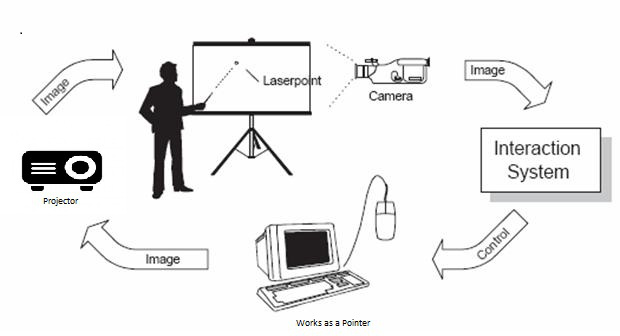
\includegraphics[scale=0.7]{abc}
%\caption {Laser Pointer based Interactive Projector System}
%\end{figure}
%2222222222222222222222222222222222222222222222222222222222222222222222222222
\clearpage
\newpage
\section{LITERATURE REVIEW}
The current prototype can run off a rechargeable 12V battery, has the capability to access the World Wide Web(WWW), has readily available off line content, via established partnerships, and has an extremely easy to use interface. The device is contained in a single unit with replaceable external components (i.e. keyboard, remotes), consumes less than 100 W of power, and will cost only USD 300. The system is about the size of a shoe-box. 
As seen in the figure, the existing Looma system functional parts can be listed as:

\subsection{Looma and Wand Details}
\begin{enumerate}
\item300 lumen projector
\item Internet Connected 
\item Wireless Wand control from front of room
\item Audio output for large room setting
\item Rechargeable 12V battery (8Hrs per charge)
\item Computer: Panda board
\item External ports: 1 Ethernet
\item Custom power supply (12V in 5V, 12V, 19.5V out)
\item Hacked Wii IR Camera and Wii wands
\end{enumerate}

\begin{figure}[htp]
\centering
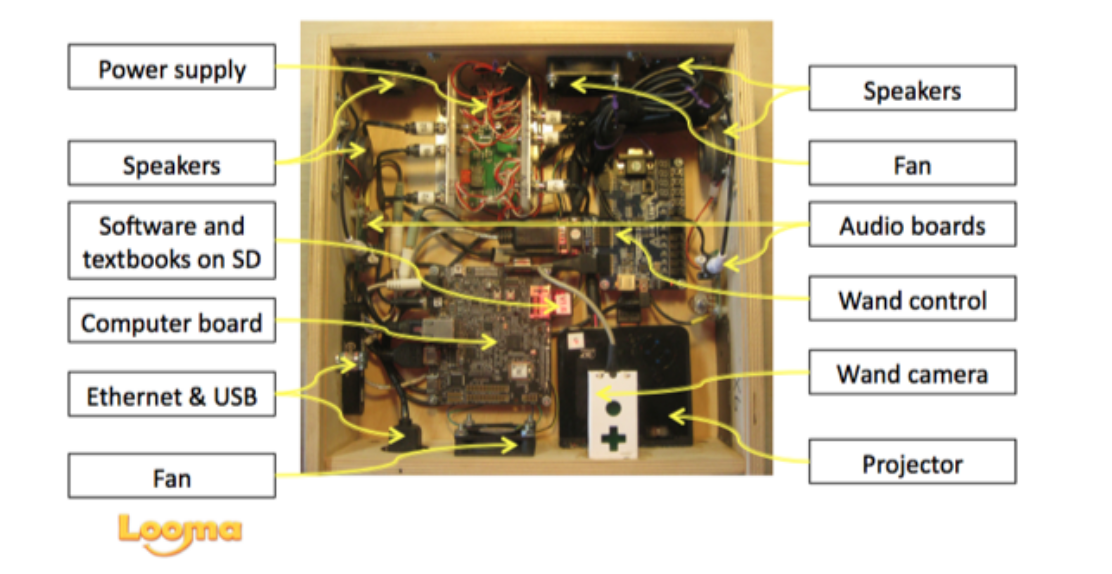
\includegraphics[scale=0.22]{looma}
\caption{Hardware and Electrical parts of Looma system}
\label{}
\end{figure}

\newpage

Wand control descriptions:
\begin{enumerate}
\item Wand shown in the figure is a 3D printed IR light source
\item The wand design uses 555 timer to turn the IR light source on/off at a pre-determined frequency such that the blink can be interpreted as a click on the device
\item Current design uses Nintendo Wii IR camera, which are scavenged from Wii motes
\end{enumerate}

\begin{figure}[htp]
\centering
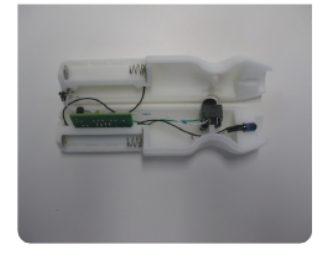
\includegraphics[width=2.4in]{wand1}
\caption{3D printed hacked Wii Remote wand}
\label{}
\end{figure}

\subsection{System Operation Description}
\begin{figure}[htp]
\centering
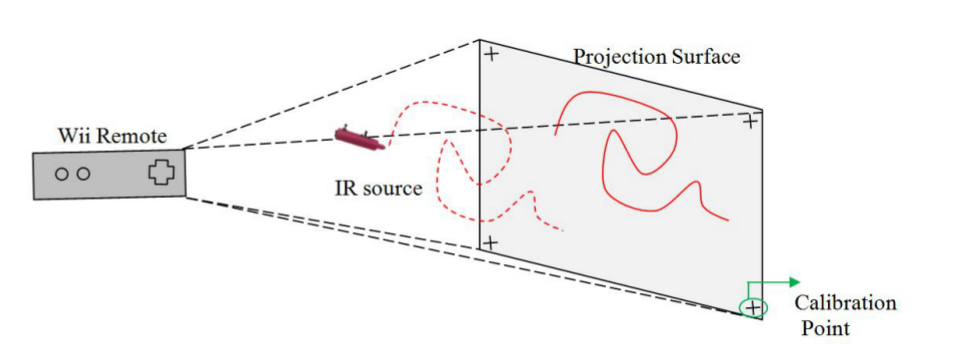
\includegraphics[scale=0.35]{wiiiii.png}
\caption{Illustration of how the movement of infrared is picked up by the Wiimote}
\label{}
\end{figure}

The existing system uses Wii Remote to interact in the audio-visual device. This system uses an Wii IR camera which picks up the infrared light source, and tracks it using its Multi-Object Tracking (MOT) processor present in the camera chip as shown in the figure. Wii IR Camera gives out a pre-set Inter-Integrated Circuit (I2C) address so the interface board needs an I2C multiplexer. To convert the I2C output to serial, and to demultiplex the signals, the system has been using an FPGA board. 
%333333333333333333333333333333333333333333333333333333333333333333333333333333
\newpage
\section{BACKGROUND THEORY}

\subsection{Basic Overview}

\subsubsection{Human-Computer-Interaction (HCI)} 
HCI is the study of how people interact with computers and to what extent computers are or are not developed for successful interaction with human beings. Developing human-computer interactions involves design on both sides of the interaction. On the technology side, the designer must have a thorough understanding of the available hardware and software components and tools. On the human side, the designer must have a good understanding of how humans learn and work with computers, including envisioning new modes of working. The designer's task is to create effective, efficient, and satisfying interactions by balancing factors such as cost, benefits, standards, and the environmental constraints in which the interaction will take place. 

Classrooms today are filled with a diverse range of students. Many of them are computer literate while others are not. Some are primarily visual learners, some are auditory learners and some kinesthetic. Others may be gifted and talented.Still others may struggle with physical, mental, behavioral or emotional challenges. In such diverse environment, it may be difficult for the teacher to cope up with each and every individual. In such cases, an effective human-computer interaction tool plays a pivotal role.Various tools are now available for the efficient human-computer interaction, one of which is the Interactive Smart Board.

The Smart Board is an interactive whiteboard that uses touch detection for user input (for example scrolling and right mouse-click) in the same way as normal PC input devices. The Smart Board interactive whiteboard operates as part of a system that includes the interactive whiteboard, a computer, a projector and whiteboarding software which can be used in various areas like offices, schools,etc.Among the various areas of application of human-computer interaction, education systems are more likely to benefit from its use.

\subsubsection{Digital Image Processing}
An image may be defined as a two-dimensional function, f(x, y), where x and y are spatial (plane) coordinates, and the amplitude of f at any pair of coordinates (x, y) is called the intensity or gray level of the image at that point. When x, y, and the amplitude values of f are all finite, discrete quantities, we call the image a digital image. The field of digital image processing refers to processing digital images by means of a digital computer.
Image processing can be defined method to convert an image into digital form and perform some operations on it, in order to get an enhanced image or to extract some useful information from it. It is a type of signal dispensation in which input is image, like video frame or photograph and output may be image or characteristics associated with that image. Usually Image Processing system includes treating images as two dimensional signals while applying already set signal processing methods to them.~\cite{raf}

The basic stages used in image processing are described as follows:
%{\begin{enumerate}
%\item Image Acquisition
%\item Image Enhancement
%\item Processing
%\item Recognition
%\end{enumerate}}

\begin{enumerate}
\item \textbf{Image Acquisition}
Image acquisition is the first stage of any vision system as all the other stages of image processing begin only after the acquiring of the digital image. It is the process in which capturing of
individual, digital still frames from an analog video signal or a digital video stream.
It is usually employed as a component of a computer vision system, in which video
frames are captured in digital form and then displayed, stored or transmitted in raw
or compressed digital form. Frame grabbers were the predominant way to interface
cameras to PC's i.e. direct camera connections via USB. The digital image is captured with the help of image sensor. An image sensor is a device that converts an optical image into an electronic signal such as, digital cameras, camera modules and other imaging devices. Here, Raspberry CSI camera is used for image acquisition.

\item \textbf{Image Enhancement}
After acquiring the image, the next stage is its enhancement. Image enhancement comprises the algorithms that make necessary changes to the original images so that they can be made more useful for further processing. For example: RGB to grayscale conversion is done to convert the 24 bit per pixel data to 8 bit per pixel data. 
When converting an RGB image to
grayscale, we have to take the RGB values for each pixel and make as output a
single value reflecting the brightness of that pixel. One such approach is to take the
average of the contribution from each channel: (R+B+C)/3. 

However, since the
perceived brightness is often dominated by the green component, a different, more human-oriented, method is to take a weighted average, e.g.0.3R + 0.59G + 0.11B. Some of the image enhancements, we have performed are such grayscale conversions, smoothing the image etc. 
Smoothing, also called blurring, is a simple and
frequently used image processing operation. There are many reasons for
smoothing. In this tutorial we will focus on smoothing in order to reduce noise
(other uses will be seen in the following tutorials).To perform a smoothing
operation we will apply a filter to our image.


\item \textbf{Processing}
After the enhancement of the image, it is processed to get the further result with the respective algorithms. Some algorithms such as canny edge detection and hough transforms are applied to the image and inferences are developed from the results obtained. Edges characterize boundaries and are
therefore a problem of fundamental importance in image processing. Edges in
images are areas with strong intensity contrasts – a jump in intensity from one pixel to the next. Edge detecting an image significantly reduces the amount of data and
filters out useless information, while preserving the important structural properties
in an image. This characteristic is utilized in the canny edge detection.

The hough transform is a feature extraction technique
used in image analysis, computer vision, and digital image processing The purpose
of the technique is to find imperfect instances of objects within a certain class of
shapes by a voting procedure. This voting procedure is carried out in a parameter
space, from which object candidates are obtained as local maxima in a so-called
accumulator space that is explicitly constructed by the algorithm for computing the
hough transform.

\item \textbf{Recognition}
Once the  processing operations are completed, the required algorithms are applied for the feature recognition such as laser detection in our case. Here, the recognised feature is the laser pointer on the projector screen.
\end{enumerate}

\subsubsection{Embedded System}
A microcontroller is a self-contained system with peripherals, memory and a processor that can be used as an embedded system. Most programmable microcontrollers that are used today are embedded in other consumer products or machinery including phones, peripherals, automobiles and household appliances for computer systems. Due to that, another name for a microcontroller is an embedded controller.

Some embedded systems are more sophisticated, while others have minimal requirements for memory and programming length and a low software complexity. An embedded system is an engineering artifact involving computation that is subject to physical constraints(reaction constraints and execution constraints) arising through interactions of computational processes with the physical world. Reaction constraints originate from the behavioural requirements, throughput, and jitter whereas execution constraints originate from the implementation requirements and put bounds on available processor speeds, power, memory and hardware failure rates. The key to embedded systems design is to obtain desired functionality under both kinds of constraints. 

Embedded systems are application specific and single functioned and efficiency is of paramount importance for embedded systems. They are optimized for energy, code size, execution time, weight and dimensions, and cost.These sysems are typically designed to meet real time constraints; a real time system reacts to stimuli from the controlled object or operator within the time interval dictated by the environment. For real time systems, right answers arriving too late (or even too early) are wrong. Also they often interact (sense, manipulate and communicate) with external world through sensors and hence are typically reactive systems; a reactive system is in continual interaction with the environment and executes at a pace determined by that environment.
They generally have minimal or no user interface. 


\subsection{Tools Used For Hardware}
\subsubsection {Proteus VSM}
The Proteus VSM contains mixed mode SPICE circuit simulation, animated components and microcontroller models to facilitate co-simulation of complete microcontroller based design. It is possible to develop and test such designs before a physical prototype is constructed. This is possible because interaction with the design is possible using circuit indicators like LED, display panels, actuators etc. It also provides extensive debugging facility by employing breakpoints, single stepping and variable display of both assembly code and high level language source code.

\subsubsection{Eagle}
Eagle is acronym for “Easily Applicable Graphical Layout” which is a flexible, expandable and scriptable schematic capture editor, PCB layout editor, auto-router and CAM and BOM tools developed by CadSoft Computer. 

\subsubsection {AVR Studio 6}
AVR Studio 6 is a software development environment developed by Atmel. It is a full software development with an editor, simulator, programmer, etc. It comes with its own integrated C compiler, the AVR GNU C Compiler (GCC). It also supports several programmers including the STK500, AVR Dragon, etc. 

\subsubsection{SinaProg}
SinaProg is Hex downloader application with AVRDude and Fuse Bit Calculator. This is used to download code/program and to set fuse bits of all AVR based microcontrollers. 

\newpage
\section{Software implementation and simulation}
\subsection{Python}

IDLE is an integrated development environment for Python, which has been bundled with each release of the language. It is packaged as an optional part of the Python packaging
with many Linux distributions. It is completely written in Python and the Tkinter GUI
toolkit (wrapper functions for Tcl/Tk).According to the included README, its main
features are:
\begin{enumerate}
\item Multi-window text editor with syntax highlighting, auto completion, smart indent
and other.
\item Python shell with syntax highlighting.
\item Integrated debugger with stepping, persistent breakpoints, and call stack visibility.
\end{enumerate}
\subsection{Open Source Computer Vision Library (OpenCV):}

OpenCV is an open-source Berkeley Software Distribution (BSD)-licensed library
that includes several hundreds of computer vision algorithms. It focuses mainly on real-
time image processing. OpenCV library has been used in python platform.
OpenCV has a modular structure, which means that the package includes several shared or
static libraries.
\begin{enumerate}
\item core - a compact module defining basic data structures, including the dense
multidimensional array Mat and basic functions used by all other modules.
\item imgproc - an image processing module that includes linear and non-linear image
filtering, geometrical image transformations (resize, affine and perspective warping,
generic table-based remapping), color space conversion, histograms, and so on.
\item video - a video analysis module that includes motion estimation, background
subtraction, and object tracking algorithms.
\item calib3d - basic multiple-view geometry algorithms, single and stereo camera
calibration, and object pose estimation, stereo correspondence algorithms, and
elements of 3D reconstruction.
\item features2d - salient feature detectors, descriptors, and descriptor matchers.
\item objdetect - detection of objects and instances of the predefined classes (for
example, faces, eyes, mugs, people, cars, and so on).
\item highgui - an easy-to-use interface to video capturing, image and video codecs, as
well as simple UI capabilities.
\item gpu - GPU-accelerated algorithms from different OpenCV modules.
It also includes some other helper modules, such as FLANN and Google test wrappers,
Python bindings, and others.
\end{enumerate}

\subsection{Tkinter:}

It is a standard builds of Python include an object-oriented interface to the Tcl/Tk widget set,
called \textbf{Tkinter}. This is probably the easiest to install and use. The Tkinter module (“Tk interface”) is the standard Python interface to the Tk GUI toolkit.
Both Tk and Tkinter are available on most Unix platforms, as well as on Windows
systems. Tcl/Tk is fully portable to the MacOS, Windows, and Unix platforms.
The Tkinter module is a thin object-oriented layer on top of Tcl/Tk. Tkinter is a set of
wrappers that implement the Tk widgets as Python classes. In addition, the internal module
tkinter provides a threadsafe mechanism which allows Python and Tcl to interact.
Tkinter‘s chief virtues are that it is fast.

\subsection{ Picamera:}

Raspberry Pi camera module can use \emph{Picamera 1.2}. It is a pure Python interace to the camera module. The interface eradicates the need to use command line syntax for grabbing image frames and videos. It does not cause restart of the camera interfaces when changing the intrinsic camera properties
. 
\subsection{ PyMouse:}
It is a pure Python cross-platform mouse control module. Mouse functions are provided by the PyMouse library. It runs on any Linux system running over X11 display server. PyMouse provides simple functions like move, click, press and release. PyMouse is a wrapper over Python X Library. It is used to move the mouse pointer as per the laser pointer movements. It is a fully functional X client library intended for Python programs, working as client to communicate with the X server via the X protocol. It runs on Linux using XFree86 as the server and most Unices.


The X Window System is a network-transparent window system that was designed at MIT. X display servers run on computers with either monochrome or color bitmap display hardware. Once the connection is set up, the Xlib macros are used to get the information about the current display. Similarly, using the X objects, the mouse pointer is moved by sending coordinates to the appropriate functions. 


\newpage
%4444444444444444444444444444444444444444444444444444444444444444444444444444
\section{SYSTEM DEVELOPMENT}
\subsection{Projected Screen of Looma}
The Looma software runs on any linux hardware. The display resolution of the screen is given by X = 1280 and Y = 768, and the display width is 60. Once the device is up, there are options of whether to use the wand or not use the wand. In the projected screen of Looma software, we are presented with teaching contents for students as shown in figure 4.1.

\begin{figure}[htp]
	\centering
		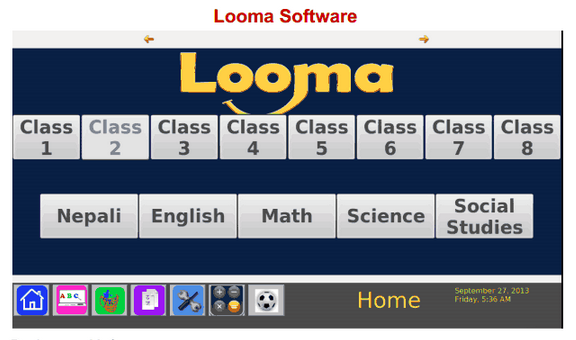
\includegraphics[scale=0.3]{loomasoftware.png}
	\caption{Looma Software}
\label{}
\end{figure}

\subsection{System Block Diagram and Description}

The images of Looma are grabbed in real time by Raspberry Pi camera board. The laser detection and click action detection algorithm is run on the Raspberry Pi.

First, the projected screen is captured and the four corners of the projected screen is obtained which is our Region of Interest(ROI). The arrangement of the raspberry pi system and looma system is made such that, the imagery of the projected screen is undistorted and unwarped. The linear mapping is done to map the image coordinates from raspberry pi to the display resolution of the computer.
\newpage

\begin{figure}[htp]
\centering
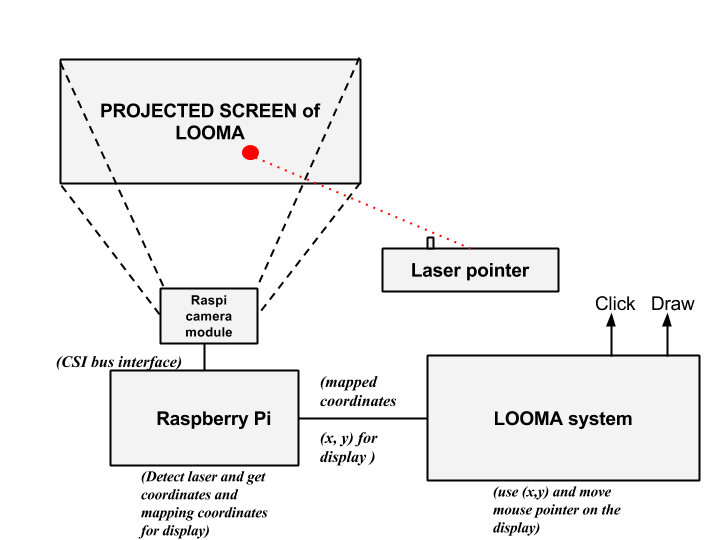
\includegraphics[scale=0.6]{proposed_system}
\caption{System Block Diagram}
\label{Block Diagram}
\end{figure}
The next task is updating mouse as per the laser point's actions. In all conditions, whenever laser point is seen inside the projected screen, the mouse pointer move command is given to the system using the projector. In the case of blinks of laser point, click or drag actions is given based on the number of clicks. 

The communication between raspberry pi and the computer system is done via client server architecture as shown in the Appendix A.1.
%5555555555555555555555555555555555555555555555555555555555555555
\newpage
\section{METHODOLOGY}
The main purpose of the reformed wand is to establish a way of interaction between the user and the projector system. Hence, this system needs to accomplish the following tasks to overcome the limitations provided by the current Looma wand system:
\begin{enumerate}
\item Get sequence of frames from the real-time video of the projected screen
\item Use of laser light instead of infra-red for greater flexibility in the use of mouse pointer
\item Detect laser’s on or off states in each frame using image processing algorithms
\item Based on the results of detection, generate appropriate mouse press and release actions to operate mouse
\end{enumerate}

\subsection{Initial Calibration of Projected Screen}
	 The projected screen is our region of interest. The four corners of the projected screen are first extracted, which is where we want our laser point to be detected within. 
%\begin{figure}[htp]
%	\centering
%	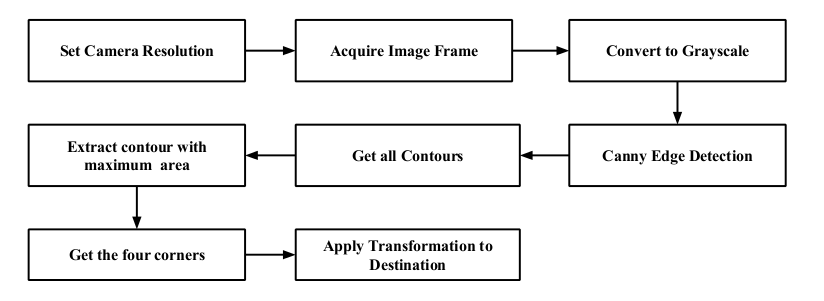
\includegraphics[scale=0.50]{Calibration.png}
%	\caption{Calibration Process}
%	\label{}
%\end{figure}
	 
    The projected screen is distinguished from the wall surface by applying a threshold on the grayscale image. The applied threshold binarized the captured image such that, the grayscale image is turned into a binarized image. The projected screen is thresholded into a white surface and the rest of the image is seen as black. The contour finding algorithm is applied to this image. The contour with the largest area, which is the projected screen is obtained. The rectangular approximation of this contour gives the x and y coordinates of the projected screen. 
 
    The obtained coordinates are in the image plane coordinate system, which needs to be mapped to the projected computer’s screen coordinates. First of all, the x and y coordinates of the obtained projected screen is translated to the origin of the image plane coordinate 
The mapping is based on linear mapping technique which works on the straight undistorted projection. 

\begin{figure}
\centering	 
\tikzstyle{decision} = [diamond, draw, text width=4.5em, text badly centered, node distance=3cm, inner sep=0pt]
\tikzstyle{block} = [rectangle, draw, text width=6em, text centered, rounded corners, minimum height=4em]
\tikzstyle{line} = [draw, -latex']
\tikzstyle{cloud} = [draw, ellipse, node distance=3cm,
    minimum height=2em]
\tikzstyle{circle} = [draw, ellipse, node distance=3cm,
    minimum height=2em]
\begin{tikzpicture}[node distance = 2cm, auto]
    % Place nodes
    
    \node [block, node distance=4cm] (Set) {Set Camera Resolution};

    \node [block, right of=Set, node distance=4cm] (Acquire) {Acquire Image Frame};
    
    \node [block, right of=Acquire, node distance=4cm] (Convert) {Convert to Grayscale};
    
    \node [block, below of=Convert, node distance=3cm] (Canny) {Canny Edge Detection};
    \node [block, left of=Canny, node distance=4cm] (Get) {Get all Contours};
    
    
    \node [block, left of=Get, node distance=4cm] (Extract) {Extract contour with maximum area};
    
    \node [block, below of=Extract, node distance=3cm] (Get1) {Get the four corners};
    
    \node [block, right of=Get1, node distance=4cm] (Apply) {Apply Transformation to Destination};


    % Draw edge
    \path [line] (Set) -- (Acquire);            
    \path [line] (Acquire) -- (Convert); 
    \path [line] (Convert) -- (Canny);
    \path [line] (Canny) -- (Get);
    \path [line] (Get) -- (Extract);
    \path [line] (Extract) -- (Get1);
    \path [line] (Get1) -- (Apply);
  
\end{tikzpicture}
\caption{System Methodology}
\end{figure}

\begin{enumerate}
\item Detection of edges to obtain the edge map using Canny edge algorithm
\item Detection of all contours
\item Get parent contour of contour with maximum area
\item Get the four corners of this parent contour
\item Apply the  transformation of these corners to a destination coordinates
\end{enumerate}

\textbf{Canny Edge detection:}
For the edge detection we used canny edge detection algorithm.It is a multi-stage algorithm and we will go through the following stages:
\begin{enumerate}
\item \textbf {Noise Reduction}
Since edge detection is susceptible to noise in the image, first step is to remove the noise in the image with a 5x5 Gaussian filter.

\item \textbf{Finding Intensity Gradient of the Image}
Smoothened image is then filtered with a Sobel kernel in both horizontal and vertical direction to get first derivative in horizontal direction (Gx) and vertical direction (Gy). From these two images, we can find edge gradient and direction for each pixel as given by the equations 5.1 and 5.2.
\begin{equation}
\text{Edge Gradient}(G) = \sqrt{Gx^2 + Gy^2}
\end{equation}
\begin{equation}
\text{Angle}(\theta) = \arctan\bigg(\frac{Gy}{Gx}\bigg)
\end{equation}
Gradient direction is always perpendicular to edges. It is rounded to one of four angles   representing vertical, horizontal and two diagonal directions.
\item \textbf{Non maximum Suppression}
After getting gradient magnitude and direction, a full scan of image is done to remove any unwanted pixels which may not constitute the edge. For this, at every pixel, pixel is checked ­if it is a local maximum in its neighborhood in the direction of gradient.

\item \textbf{Hysteresis Thresholding}
This stage decides which are all edges are really edges and which are not. For this, we need two threshold values, minVal and maxVal. Any edges with intensity gradient more than maxVal are sure to be edges and those below minVal are sure to be non-edges, so discarded. Those who lie between these two thresholds are classified edges or non-edges based on their connectivity. If they are connected to “sure-edge” pixels, they are considered to be part of edges. Otherwise, they are also discarded.
\end{enumerate}
	
\subsection{Detection of Laser Pointer}
	Since the projected screen can comprise of all sorts of colored imagery, color based segmentation method is not appropriate for the detection of laser. For flawless detection of laser, the exposure of the camera is programmatically reduced so that laser is the only brightest pixel seen in the image frame. 
	\subsubsection{Dynamic Exposure Correction}
	A photograph's exposure determines how light or dark an image appears when it is captured by the camera. 
	
	The Raspberry Pi's camera is programmable. The camera's capture property is controlled by the camera exposure compensation parameter. The exposure correction is done as per the captured image's property dynamically. 
	
	The proper exposure configuration improves the detection of the laser. After the projected screen is captured, and the camera exposure values are modified until the laser spot is the brightest in the input image. On every frame captured, the average of the value channel of the image is compared with the preset threshold and the camera exposure level is decreased accordingly if the average value of channel is greater than this threshold.
	
	
\subsubsection{Brightest Pixel Detection}
After exposure compensation is done based on the average value of the image captured, the steps involved in detecting the brighest pixel area and its location can be described in the following points:
\begin{enumerate}
\item {\textbf{Grayscale conversion}}
Grayscale image carries the intensity information. It is composed of shades of gray, varying from black at weakest intensity to white at the strongest. 

A RGB image is captured by Rpi at first, which contains all the three components: Red (R), Green (G), Blue (B). The processing of all these components is redundant and time inefficient. The grayscale conversion is done so that the RGB values are expressed by intensity values within a given range of 0 to 255 values. These grayscale levels are then thresholded by binary thresholding algorithm. 
\newpage
\item {\textbf{Binary Thresholding}}

It is a segmentation method. Thresholding application involves separating out regions of an image corresponding to objects which is to be analyzed. This separation is based on the variation of intensity between the object pixels and the background pixels.

To differentiate the pixels we are interested in from the rest (which will eventually be rejected), we perform a comparison of each pixel intensity value with respect to a threshold (determined according to the problem to solve). Here, we have set the threshold to be 200 such that regions above this value is thresholded as white and rest of the pixels are thresholded as black.


\item {\textbf{Find Contours}}
Contours can be explained simply as a curve joining all the continuous points (along the boundary), having same color or intensity. Before finding contours, threshold or canny edge detection should be applied. And it outputs the contours and hierarchy.
The outermost contour is taken as laser.

\item{\textbf{Approximate by a bounding rectangle}}
The obtained contour is then approximated by a bounding rectangle which gives us the x, y coordinates as well as the width and height of the laser. This is then used to move the mouse pointer. 

\end{enumerate}
		
\subsection{Microcontroller to generate laser pulses}

	An AVR microcontroller is used instead of 555 timer so that resistor and capacitors values need not be changed with the change in frequencies and duty cycles. Below, is the schematic of the system circuit. The laser is turned on when the supply is applied. When the push button is pressed, a pulse at a frequency set to 6Hz in the microcontroller. The schematic diagram of our circuit can be followed below, and the schematic as well.
	

\begin{figure}[htp]
	\centering
	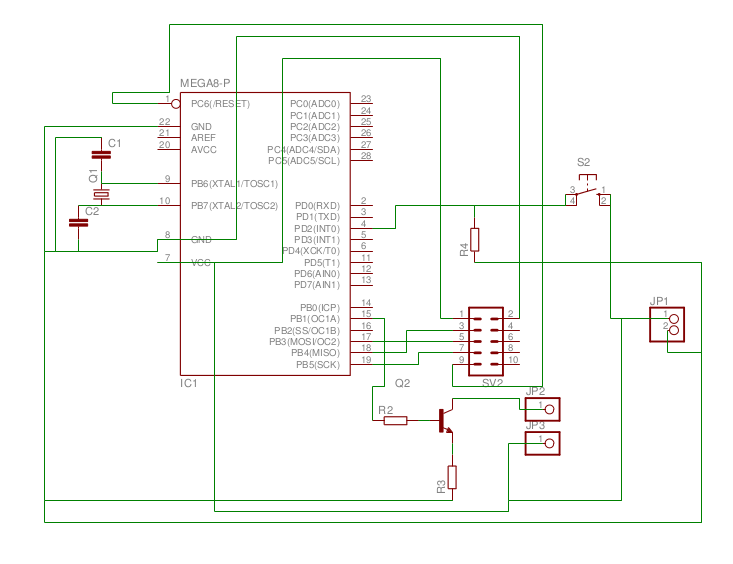
\includegraphics[scale=0.55]{schematic.png}
	\caption{Laser circuit schematic diagram}
	\label{}
\end{figure}

\begin{figure}[htp]
	\centering
	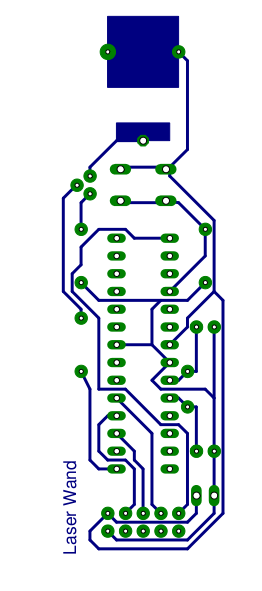
\includegraphics[scale=0.3]{eagle-non-mirror.png}
	\caption{Laser circuit eagle design diagram}
	\label{}
\end{figure}

	The laser circuit has been programmed such that it produces a 6Hz pulses when the push button is pressed, else it stays on. The target frequency has been set to 6Hz. The prescaler used is 64. The top value for pulse width modulation(PWM) is obtained as in the following equation 5.3. 
	\begin{equation}
	Top\ value = (Clock\  frequency/Target\  frequency)*Scaler - 1
	\end{equation}
	
	The top value is 20833. For a 20 per cent duty cycle, the on time of the laser is set to 20 per cent of the top value and off time is set to the 80 per cent of the top value. We have kept the push button switch in the interrupt pin, so that when the button is pushed, interrupt is obtained and the subsequent Interrupt Service Routine(ISR) can be run. This ISR does the work of producing PWM pulses of 20 per cent duty cycle. The diagram below is our working circuit.

\begin{figure}[htp]
	\centering
	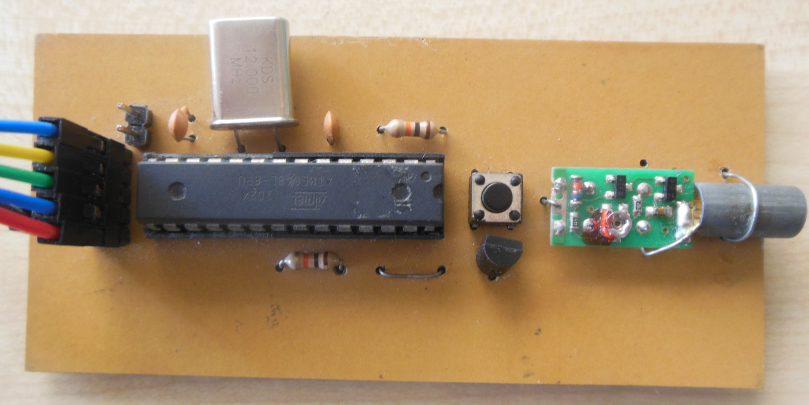
\includegraphics[scale=0.2]{front.png}
	\caption{Laser circuit fabricated design}
	\label{}
\end{figure}

\subsection{Hardware Implementation}
\subsubsection{Laser Wand}

A laser wand is the main interacting tool with the vision-based interactive projector system. The laser wand is a custom designed and self fabricated AVR Atmega 8L (pin diagram shown in Appendix A ) microcontroller based system. The input to the wand is a manual button press and outputs from the wand are either continual or varying laser blinks. 

On continual button press, the blinking of laser wand is made to occur at 6Hz with duty cycle of 20 per cent. Duty cycle is the ratio of on-time of a signal to the total time of a signal. The total time of a signal is the sum of on-time and the off-time of the signal. The on-time is the window frame of the signal, where the signal is high and off-time is the window frame of the signal, where the signal is low. So a duty cycle of 20 per cent implies that laser is on 20 per cent of the time and off 80 per cent of the time when the button is pressed. 

\subsubsection{Components of Laser Wand}

\subparagraph{Laser}

Laser is a device that emits light by optical amplification based on stimulated emission of electromagnetic radiation. The term \textbf{LASER} is originated as an acronym for \textbf{L}ight \textbf{A}mplification by \textbf{S}timulated \textbf{E}mission of \textbf{R}adiation. Laser light is different from other sources of light because it emits light coherently, thus allowing light to be focused on a tight spot. The laser light being used is of class IIIA, whose power output is 4mW and gives out light of wavelength 630-680nm. 

\subparagraph{Microcontroller}

The laser wand is made to blink on manual press of a button. The microcontroller has three timers 0, 1, 2 of which 16 bit timer 1 is used in non-inverting PWM mode. The prescaler is set to 64. The Timer and PWM of the avr microcontroller is used to achieve that (pin diagrams are shown in Appendix B).

\subsection{Finalized algorithm for click and drag}
	We constructed a State Diagram with the following states of laser.
	\begin{figure}
\centering
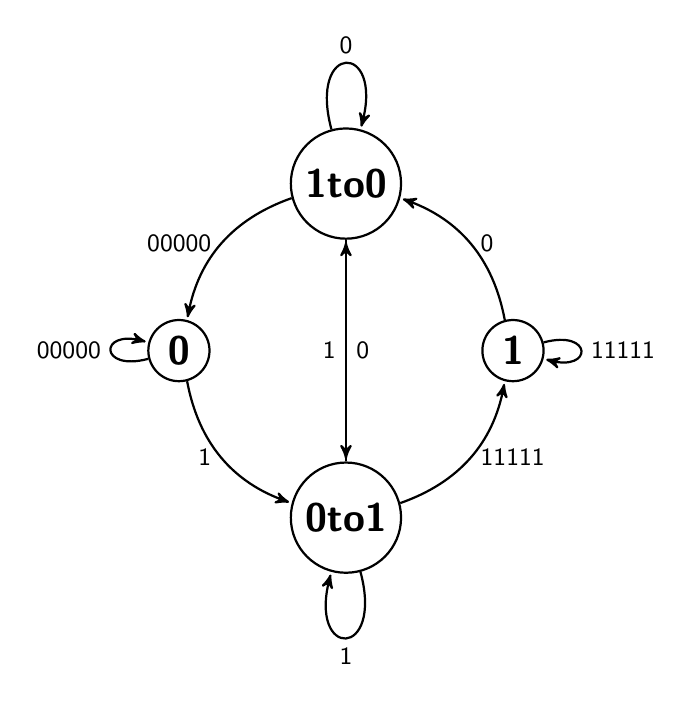
\begin{tikzpicture}[->,>=stealth',shorten >=1pt,auto,node distance=3cm,
  thick,main node/.style={circle,draw,font=\sffamily\Large\bfseries}]

  \node[main node] (1) {1to0};
  \node[main node] (2) [below left of=1] {0};
  \node[main node] (3) [below right of=2] {0to1};
  \node[main node] (4) [below right of=1] {1};

  \path[every node/.style={font=\sffamily\small}]
    (1)
        edge [bend right] node[left] {00000} (2)
        edge [loop above] node {0} (1)
        edge node [left] {1} (3)
    (2) 
        edge [loop left] node {00000} (2)
        edge [bend right] node[left] {1} (3)
        
    (3) edge node [right] {0} (1)
        edge [bend right] node[right] {11111} (4)
        edge [loop below] node {1} (3)
    (4) 
        edge [loop right] node {11111} (4)
        edge [bend right] node[right] {0} (1);
\end{tikzpicture}
\caption{State Diagram}
\end{figure}
\begin{enumerate}
\item Laser-off or 0
\item Laser-on or 1
\item Toggle 0to1 or 1to0 
\end{enumerate}

	\textbf {Laser-off} is a state of continual five or more laser-off  states, which occurs when the laser is not detected. \textbf{Laser-on} is a state of continual five or more laser-on states, when the laser is detected. \textbf{Toggle-0to1} occurs when laser state is toggled from off state to on state, whereas in \textbf{Toggle-1to0}, laser state is toggled from on state to off state. 
	
	At all times, when laser is in the on state, the mouse pointer is continually updated to move. When laser state is toggled, either from laser on to off or vice-versa, the mouse pointer is pressed. If the mouse pointer is moved while in pressed state, drag occurs. This continues until a laser-off state or laser-on state occur, which is interpreted as a mouse release. And, at every toggle state, mouse down occurs and if laser-on or laser-off state is immediately succeeded to this event, then mouse is released which is then interpreted as click and the states can be viewed in the figure 5.5 and the flowchart for the algorithm is given in the Appendices J.1 and J.2.

%\begin{figure}[htp]
%\centering
%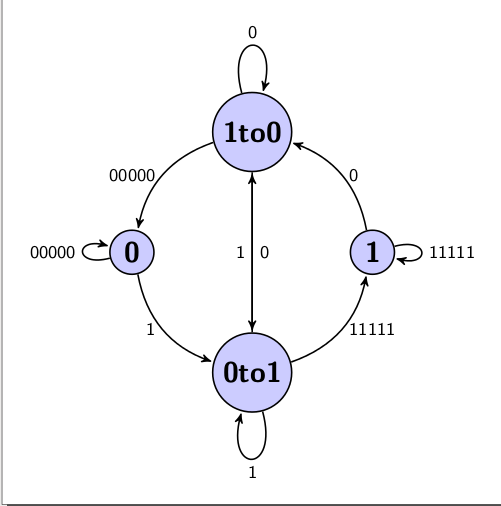
\includegraphics[scale=0.35]{state.png}
%\caption{State Transition Diagram of Algorithm}
%\label{}
%\end{figure}	
\subsection{Communication between computer and Raspberry Pi}
	A server and client program are constructed based on TCP protocol. The server and client maintain the communication between the computer and the raspberry pi. The server program is run on the computer which is being projected by the projector. The client program is run on the raspberry pi which detects laser spots. 
	
	Currently, the Looma software is obtaining the mouse coordinates through its serial port from the FPGA board. So we have implemented a protocol for communication using TCP protocol to communicate the mouse actions and coordinates to the computer. The Looma board is made a server, and the Raspberry Pi board a client. The client sends the coordinates of the detected laser spot, and the actions associated with it. Accordingly, the server which is listening to the client, receives the coordinates and their respective actions. The server then sends the actions to the in-built mouse application to do the desired action.  For the basic TCP protocol diagram, see Appendix A.1.


\subsection{Movement of Mouse Pointer}
The laser coordinates, x and y, detected by the RPi camera is mapped to the system coordinates. 

First of all, a point obtained in the image window with width of 640 and height of 480, is translated to the origin of the image coordinates system using the following equation:

\begin{equation}
x' = x - tx
\end{equation}

\begin{equation}
y' = y - ty
\end{equation}

where tx and ty are the translation factors.

Now, the obtained point in the origin of the image window is scaled as per the scaling factor obtained as below:

A point at position (xw,yw) in the image window is mapped into position (xv,yv) in the viewport of system. To maintain the same relative placement in the viewport as in the window, we require that

\begin{equation}
 (xv -xv_{min})/(xv_{max} – xv_{min}) = (xw – xw_{min})/(xw_{max} – xw_{min})
\end{equation}
which gives the scaling factores in x and y directions as,
\begin{equation}
sx = (xv_{max} – xv_{min}) / (xw_{max} – xw_{min})
\end{equation}
\begin{equation}
sy = (yv_{max} – yv_{min}) / (yw_{max} – yw_{min})
\end{equation}

where, sx and sy are the scaling factors~\cite{hen}
The vmax and vmin are the maximum and minimum coordinates of the viewport system whereas wmax and wmin are the maximum and minimun coordinates of the image window. 
The corresponding scaling factors are multiplied to the translated image window coordinate and then re-translated using the following equations. 

\begin{equation}
x' = x + tx
\end{equation}

\begin{equation}
y' = y + ty
\end{equation}

where tx and ty are the translation factors.

The final coordinate is used to move the mouse pointer on the projected screen. 
\newpage
%6666666666666666666666666666666666666666666666666666666666666666666666666666
\section{PROBLEM FACED and SOLUTIONS}
\subsection{Laser Hardware}
Initially, in an attempt to reduce the costs of the overall laser hardware, we had attempted to pulse the laser led using 555 timer circuits. The 555 timer circuits comprised of resistors and capacitors which were picked up precisely enough to give us the required frequency. However, continual error checking and correction, for the detection of the pulsed laser led by camera, the resistors and capacitors had to be changed frequently, which proved to be inefficient and tedious.


Despite the cost constraints, we moved on to atmega 8L microcontrolle. We would have used an ATTiny45 microcontroller, which is about the same size as a 555 timer, but it was not readily available. Thereby, we programmatically pulsed our laser led, as required. Thus, it was easy to setup the laser hardware for the detection system.

In the end, we designed and fabricated the hardware, based on this microcontroller.


\subsection{Detection of laser point by HSV Segmentation}

HSV Segmentation deals with the natural color of the object to be detected. We tried to detect the laser utilizing its distinct intensity value in the red region. However, the detection failed in cases when other points with same color and intensity came on the projected screen.

For resolving the problem, we considered only the brightest pixels in the projected screen. However, along with the laser pointer, other bright parts of the view port such as the white parts of the projection itself, and other bright reflections were also being captured. So we programmatically checked the intensity of lights reaching the camera's aperture, and if it exceeded a calibrated level, we reduced the shutter time thereby only allowing minimal exposure to the image. It was found that, laser was seen to be the brightest spot among all pixels. So, an exposure correction of the camera was carried out before the start of the detection. This ensured that only the bright laser pointer is detected.
\newpage
%777777777777777777777777777777777777777777777777777777777777777777777777777777
\section{RESULTS AND ANALYSIS}

\subsection{Hardware Testing}

This phase of the hardware testing includes the following tests:
\begin{enumerate}
\item Connectivity testing
\item Cold solder testing
\item Checking the polarity of the capacitors
\item Testing the response of button and microcontroller
\end{enumerate}

\subsubsection{Testing the Laser Circuit}

The laser wand was tested by connecting the circuit elements as shown in the figure. 5.2. In the microcontroller, Pin 1 (OC1A) and Pin 2 (OC1B) of Port B were configured in PWM setting. However, instead of laser led, a normal red-led was used. 

Since a microcontroller is not a good source for external circuits, an NPN transistor was used to sink the red led to the microcontroller. And, the button to control the PWM output from the Port B pins was connected to interrupt pin at Port D, pin 2, so that on manual button presses, the led started pulsing at the desired frequency.

\begin{figure}[htp]
\centering
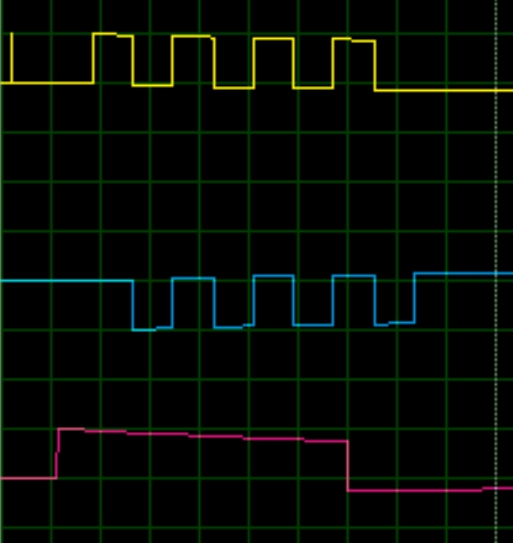
\includegraphics[scale=0.30]{afterpress.png}
\caption{PWM generation on button click}
\label{}
\end{figure}

When the button is pressed, the button gives a high on the pin 2 because it is switched from sinked state to source state at this time, which is given by the lower line in the figure 7.1. In this figure, the pwm signals from pin 1 are shown by the upper two lines.

 

\subsection{Software Testing}
\subsubsection{Algorithm Test}
In normal clock mode, a raspberry had a clock frequency of 700MHz, therefore a general laptop with a clock frequency of over 1 GHz, has better computing power. Before all the hardwares were made available to us, we initially, tested our laser detection algorithms on our computer. The inbuilt webcam or even a cheap USB webcam used with the computer do not have the programmatic exposure correction features, which raspberry pi camera had. For the purpose of testing, we used a darkly lit room and less intense projected screen for the detection of the laser point. The videos were processed in real time and the mouse down and releases were achieved in almost real time. 

	The algorithm was tested on raspberry pi by programmatically setting the exposure. The projected screen before programmatic exposure correction is given by in the top left window named \emph{Thresh} in the image shown in the Appendix B.1. This window named \emph{Thresh} is showing the projected screen as seen by the raspberry pi camera. After the exposure correction is done, only the laser pointer is the visible white dot in the window named \emph{Thresh}. The exposure corrected image in the window \emph{Thresh} can be viewed in the Appendix C.1.

\subsubsection{System Test}

The laser detection algorithm was tested on Raspberry Pi. For the communication of the detection system and the computer, a client server architecture was implemented where Raspberry Pi, being the client and the Looma’s existing Pandaboard, running as the server. In this way, the testing was carried out.

Raspberry Pi's processor is not capable of processing real time video at 24 fps. It was observed that at maximum, it processes the video at four fps. Hence, it hindered the laser detection algorithm significantly. The laser on-offs were not seen as the expected by the algorithm. Thereby, the processing  is slower than in computer where the video was being processed at 24 fps. Therefore, the overall detection and actions are not performed in real time by our system.

\newpage
%888888888888888888888888888888888888888888888888888888888888888888888888
\section{COST ANALYSIS}
\subsection{Cost Comparison between Looma System and Our System}
\begin{table*}[ht]
\begin{tabular}{|c|c|c|c|c|}
\hline
	S.N  & Existing System & Cost & Designed System & Cost\\
\hline
	1 & FPGA Board and Wiring & \$117 & Raspberry Pi & \$64.90\\
\hline
	2 & Nintendo Wii Remote & \$68.89 & Raspberry Pi Camera Module & \$29.95 \\
\hline
	3 & 3D Printed IR Wands & \$20 & Laser Pointer & \$0.9\\
\hline
	4 &  &  & Atmega8L & \$1.87\\
\hline
	 & Total & \$205.89 & Total & \$97.62\\
\hline
\end{tabular}
\caption{Cost Comparison between Existing System and Our System}
\label{tb:sw}
\end{table*}

Since Looma system is intended for the rural areas, the system needs to be as economic as possible. From the table 8.1, it can be inferred that, the system that we have designed is cheaper as compared to the existing system of Looma. Also, the overall cost of our project can be viewed in the table 8.2.
\clearpage
\subsection{Total Cost of Our Project}
\begin{table*}[ht]
\begin{tabular}{|c|c|c|c|c|}
\hline
	S.N & Items & Rate(Rs) & Quantity & Total(Rs) \\
\hline
	1 & Hydrogen Peroxide & 30 & 1 & 30 \\
\hline
	2 & Soldering Rod Bit(40W) & 250 & 1 & 250 \\
\hline
	3 & Capacitors & 10 & 2 & 20 \\
\hline
	4 & Push Button Switch & 5 & 1 & 5 \\
\hline
	5 & 12 Mhz Crystal & 35 & 1 & 35 \\
\hline
	6 & IC Base & 10 & 2 & 20 \\
\hline
	7 & Transistor & 35 & 1 & 35 \\
\hline
	8 & Drill Bit & 20 & 1 & 20 \\
\hline
	9 & PCB & 300 & 1 & 300 \\
\hline
	10 & Laser & 90 & 1 & 90 \\
\hline
	11 & Conc. HCl(250ml) & 500 & 1 & 500 \\
\hline
	12 & Aceton(250ml) & 300 & 1 & 300 \\
\hline
	13 & Atmega8L & 180 & 1 & 180 \\
\hline
	14 & Raspberry Pi & 6380.319 & 1 & 6,380.319 \\
\hline
	15 & Raspberry Pi Camera Module & 2,944.3845 & 1 & 2944.3845 \\
\hline
	16 & Laser Pointer &  0.9 & 1 & 88.479 \\
\hline 
    17 & Atmega8L & 183.8397 & 1 & 183.8397 \\
\hline
	18 & Documentation &  4000 & 1 & 4000 \\
\hline
	19 & Battery Pack & 200 & 1 & 200 \\
\hline 
    20 & Battery Holder & 50 & 1 & 50 \\
\hline 
	   & Total & & 22 & 15,443.5432\\
\hline	   
\end{tabular}
\caption{Total Cost of Our Project}
\label{tb:sw}
\end{table*}
%\clearpage
\newpage
%99999999999999999999999999999999999999999999999999999999999999999
\section{LIMITATIONS AND FUTURE ENHANCEMENTS}
\subsection{Limitations}

\begin{enumerate}
\item Due to the slow processing speed of the raspberry pi used, there is lag in the overall system. 
\item This system may not respond well under bright light conditions.
\item Since the raspberry pi camera is not permanently fixed to the system, a slight movement changes the calibration data of the system.

\end{enumerate}

\subsection{Enhancements}
\begin{enumerate}
\item A proper hardware with the raspberry pi system fixed inside Looma can prevent the system to be re-calibrated each time it is moved during use.
\item A better processor than the raspberry pi can be used to enhance the system’s speed and efficiency, allowing it to perform real time operations.
\item The system performs single clicks and drag as required by the Looma system, but with further enhancements, it can be made to perform double clicks.
\end{enumerate}
\newpage
%1000000000000000000000000000000000000000000000000000000000000000000000000000
\section{CONCLUSION}
\subsection{Conclusion}
The project \emph{Laser Pointer based Human Computer Interaction using Computer Vision} aims to provide an alternative solution to the interactive wand system developed by Looma. The system that we have designed allows the user to control the projected system from a considerable distance using the laser pointer. This aids in the teaching process and makes the audio visual learning environment more interactive. Although initially, the system had been designed to work on Looma system but we have tried to make it as generic as possible and can be used for other projector systems as well. 

   The system emphasizes on the algorithms for the detection of laser pointer on the screen and implementation of click  and drag operations. By integrating the algorithm with the proper laser hardware, the required laser pointer based interaction system has been developed successfully. The system has been tested in the real working environment. Even though the system cannot process real-time data and lags in time due to the low processing power of the raspberry pi processor. However, the required main functions are efficiently performed by the system. With enhancements suggested above, the system's accuracy and speed can be increased considerably. 
   
   During the process of development, many research works carried out in the respective fields were thoroughly studied. Based on the results and conclusions of these papers, the algorithms that best suited the domain of this project was selected and their citations can be viewed in the references.
   
   
\newpage
\renewcommand{\refname}{REFERENCES}
\begin{thebibliography}{}
	\bibitem{kir} Kirstein and Muller, Interaction with a Projection Screen Using a Camera-Tracked Laser Pointer,University of Dortmund, Germany 
	

	\bibitem{joh} Johnny Chung Lee, Hacking the Nintendo Wii Remote, Carnegie 		   Mellon University, IEEE-CS,2008 

	
	\bibitem{raf} Rafael C. Gonzalez and Richard E. Woods, Digital Image Processing, 3rd Edition
	
	\bibitem{hen} Donald Hearn and M. Pauline Baker, Computer Graphics C Version, 2nd Edition 
\end{thebibliography}

\newpage
\begin{appendices}
\section{TCP protocol}
\begin{appendixfig}
\centering
\tikzstyle{decision} = [diamond, draw, text width=4.5em, text badly centered, node distance=3cm, inner sep=0pt]
\tikzstyle{block} = [rectangle, draw, text width=7em, text centered, rounded corners, minimum height=2em]
\tikzstyle{line} = [draw, -latex']
\tikzstyle{cloud} = [draw, ellipse, node distance=3cm,
    minimum height=2em]
\tikzstyle{circle} = [draw, ellipse, node distance=3cm,
    minimum height=2em]    
\begin{tikzpicture}[node distance = 2cm, auto]
    % Place nodes
    \node [block, node distance=4cm] (Socket) {Socket()};
    \node [block, node distance=2cm, below of=Socket] (Bind) {Bind()};
    \node [block, node distance=2cm, below of=Bind] (Listen) {Listen()};
    \node [block, node distance=9cm, right of=Listen](Socket1) {Socket()};
    
    \node [block, node distance=2cm, below of=Listen] (Accept) {Accept()};
    \node [block, node distance=2cm, below of=Accept] (Block) {Block until there are connections from client};
    \node [block, node distance=9cm, right of=Block](Connect1) {Connect()};
    \node [block, node distance=2cm, below of=Block] (Read) {Read()};
    \node [block, node distance=9cm, right of=Read](Write1) {Write()};
    \node [block, node distance=2cm, below of=Read] (Write) {Write()};
    \node [block, node distance=9cm, right of=Write](Read1) {Read()};
    \node [block, node distance=2cm, below of=Write] (Close) {Close()};
    \node [block, node distance=9cm, right of=Close](Close1) {Close()};

    % Draw edge

  \path [line] (Connect1) -- node {Connection Established}(Block);
  \path [line] (Write1) -- node{Data(Request)}(Read);
  \path [line] (Write) -- node{Data(Reply)}(Read1);
  \path[line](Socket)--(Bind);
  \path[line](Bind)--(Listen);
  \path[line](Listen)--(Accept);
  \path[line](Accept)--(Block);
  \path[line](Block)--(Read);
  \path[line](Read)--(Write);
  \path[line](Write)--(Close);
  
  \path[line](Socket1)--(Connect1);
  \path[line](Connect1)--(Write1);
  \path[line](Write1)--(Read1);
  \path[line](Read1)--(Close1); 
\end{tikzpicture}
\caption{Transmission Control Protocol between Server and Client}
\end{appendixfig}
\newpage
\section{Projected Screen Before Exposure Correction}
\begin{appendixfig}
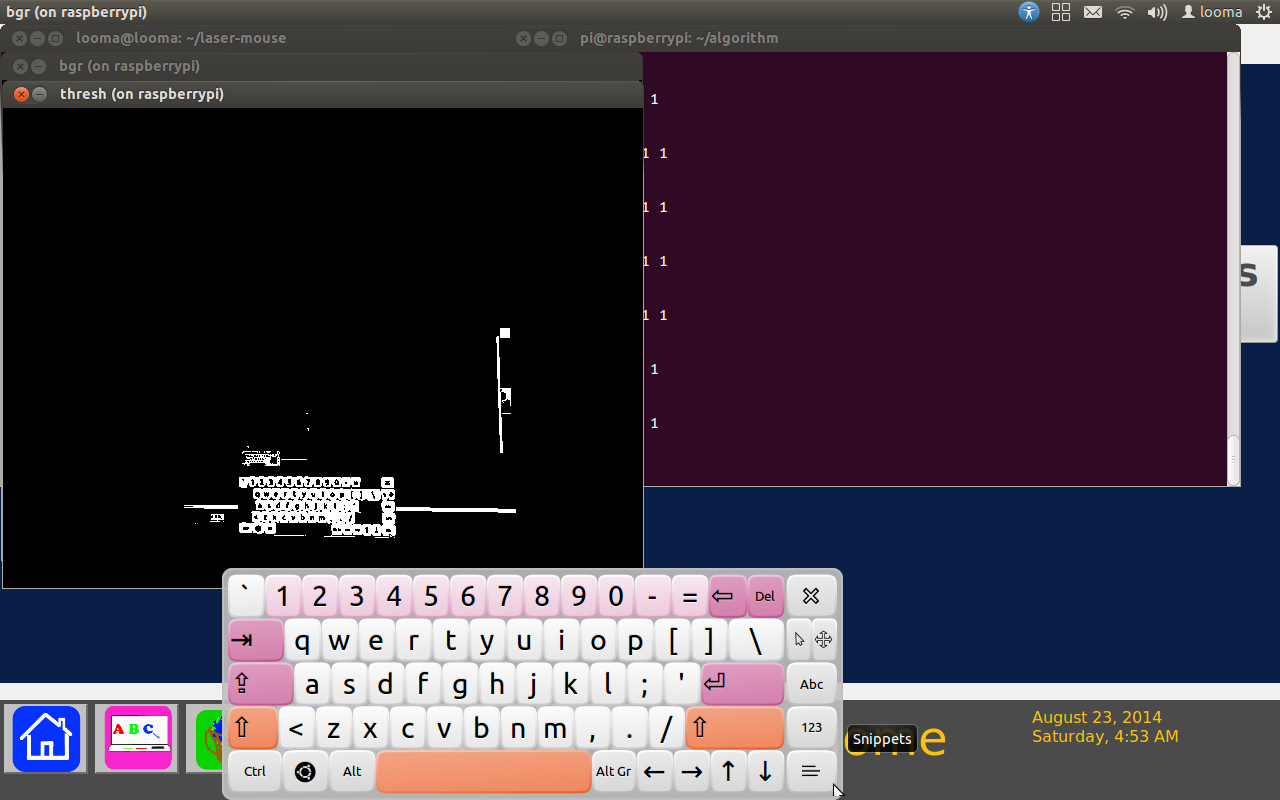
\includegraphics[scale=0.30]{projector.png}
\caption{Projected Screen Before Exposure Correction}
\label{}
\end{appendixfig}
\newpage

\section{Projected Screen After Exposure Correction}
\begin{appendixfig}
%\begin{figure}
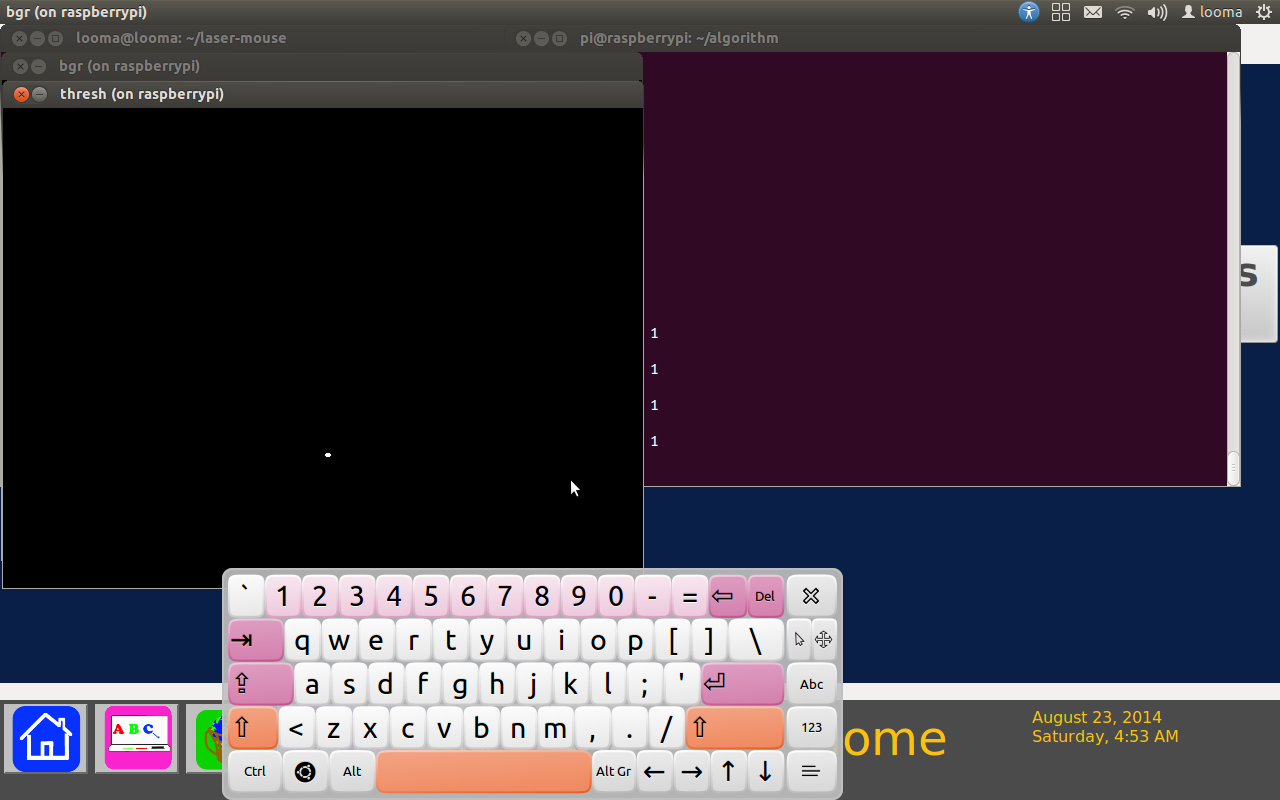
\includegraphics[scale=0.30]{projectorwithout.png}
\caption{Projected Screen After Exposure Correction}
\label{}
\end{appendixfig}
\newpage
\section{AVR Atmega 8L Features:}
\begin{enumerate}
\item \textbf{High-performance, Low-power Atmel AVR 8-bit Microcontroller}
\begin{enumerate}
\item Advanced \ac{RISC} Architecture
\item 130 Powerful Instructions – Most Single-clock Cycle Execution
\item 32 × 8 General Purpose Working Registers
\end{enumerate}
\item \textbf{High Endurance Non-volatile Memory segments}
\begin{enumerate}
\item 8Kbytes of In-System Self-programmable Flash program memory
\item 512Bytes EEPROM
\item WriteErase Cycles: 10,000 Flash. 100,000 \ac{EEPROM}
\item Data retention: 20 years at 85$^oC$ 100 years at 25$^oC$
\end{enumerate}
\item \textbf{Peripheral Features}
\begin{enumerate}
\item Two 8-bit Timer/Counters with Separate Prescaler, one Compare Mode
\item One 16-bit Timer/Counter with Separate Prescaler, Compare Mode, and Capture Mode
\item Real Time Counter with Separate Oscillator
\item Three PWM Channels
\end{enumerate}
\item \textbf{Operating Voltages}
\begin{enumerate}
\item 2.7V - 5.5V (ATmega8L)
\item 4.5V - 5.5V (ATmega8)
\end{enumerate}
\item \textbf{Speed Grades}
\begin{enumerate}
\item 0 - 8MHz (ATmega8L)
\item 0 - 16MHz (ATmega8)
\end{enumerate}
\item \textbf{Power Consumption at 4Mhz, 3V, 25$^oC$}
\begin{enumerate}
\item Active: 3.6mA
\item Idle Mode: 1.0mA
\end{enumerate}
\end{enumerate}
\newpage

\section{AVR Atmega8L Pin Diagram}
\begin{appendixfig}
\centering
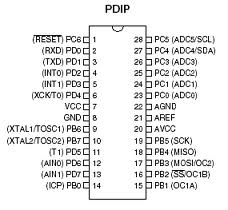
\includegraphics[scale=1.00]{avr.jpeg}
\caption{AVR Atmega8L Pin Diagram}
\label{}
\end{appendixfig}

\newpage
\section{OPENCV}
\textbf{\ac{OpenCV}} is an open source computer vision and machine learning software library. \ac{OpenCV} was built to provide a common infrastructure for computer vision applications and to accelerate the use of machine perception in the commercial products. Being a BSD-licensed product, \ac{OpenCV} makes it easy for businesses to utilize and modify the code.

The library has more than 2500 optimized algorithms, which includes a comprehensive set of both classic and state-of-the-art computer vision and machine learning algorithms. These algorithms can be used to detect and recognize faces, identify objects, classify human actions in videos, track camera movements, track moving objects, extract \ac{3D} models of objects, produce \ac{3D} point clouds from stereo cameras, stitch images together to produce a high resolution image of an entire scene, find similar images from an image database, remove red eyes from images taken using flash, follow eye movements, recognize scenery and establish markers to overlay it with augmented reality, etc.

In general, \ac{OpenCV} application areas include:

\begin{enumerate}
\item 2D and 3D feature toolkits
\item Egomotion estimation
\item Facial recognition system
\item Gesture recognition
\item Human–computer interaction HCI
\item Mobile robotics
\item Motion understanding
\item Object identification
\item Segmentation and Recognition
\item Stereopsis Stereo vision: depth perception from 2 cameras
\item Structure from motion SFM
\item Motion tracking
\item Augmented reality
\end{enumerate}
\newpage
\section{Raspberry Pi and Camera Board}
Raspberry Pi is a single-board computer with processor, memory, I/O ports and many more features, which together make it a functional computer for a wide range of applications in robotics. It is so simple than any logical person can program it, even it is for the first time when you work with a single-board computer.The ARM powered minicomputer is a platform with enormous possibilities and powerful enough to run many of the same programs as computer. Raspberry Pi serves as a wonderful platform for computer vision algorithms given its size, wonderful camera board and portability. Using the Picamera module, we took raw byte streams of the projected screen, and converted them to OpenCV (Open Computer Vision) object before doing further image processing algorithms.

Raspberry Pi Camera Board Module supports a full HD (High Definition) video streaming at fps of 30 with its 5 megapixel native resolution, and the sensor capable of 2592-1944 pixel static images. Raspberry Pi Camera Board Module was opted instead of normal USB web camera. 

The software of Raspberry Pi utilizes Rpi GPU (Graphical Processor Unit) when using Raspi Camera Module. So for example encoding \emph {h.264}, video has low impact on the CPU (Central Processor Unit) usage. Also, it has an excellent resolution of 5 Megapixels, which is higher than most USB webcams. It also has an excellent daytime image quality. If we use USB Webcam, it will have a very slow frame rate video and the CPU usage will be quite high. RPi does not have enough CPU horsepower to do higher frame rates, resolution and advanced video compression. 
\newpage
\section{Raspberry Pi Board}
\begin{appendixfig}
\centering
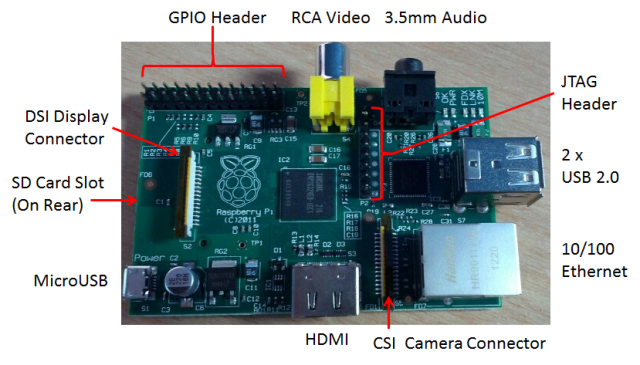
\includegraphics[scale=1.00]{RPiModelB.png}
\caption{Raspberry Pi Board}
\label{}
\end{appendixfig}

\newpage
\section{Raspberry Pi Camera Module}
\begin{appendixfig}
\centering
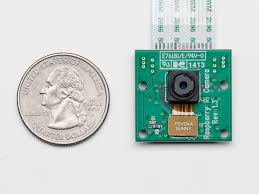
\includegraphics[scale=1.00]{index.jpeg}
\caption{Raspberry Pi Camera Module}
\label{}
\end{appendixfig}
%\newpage
%\section{TCP Protocol}
%\begin{figure}[htp]
%\centering
%\includegraphics[scale=1.00]%{tcp.png}
%\caption{Transmission Control %Protocol}
%\label{}
%\end{figure}

\newpage
%\end{figure}
%\newpage
%\\section{Flow Diagram of System}
%\\begin{figure}
%\\centering
%\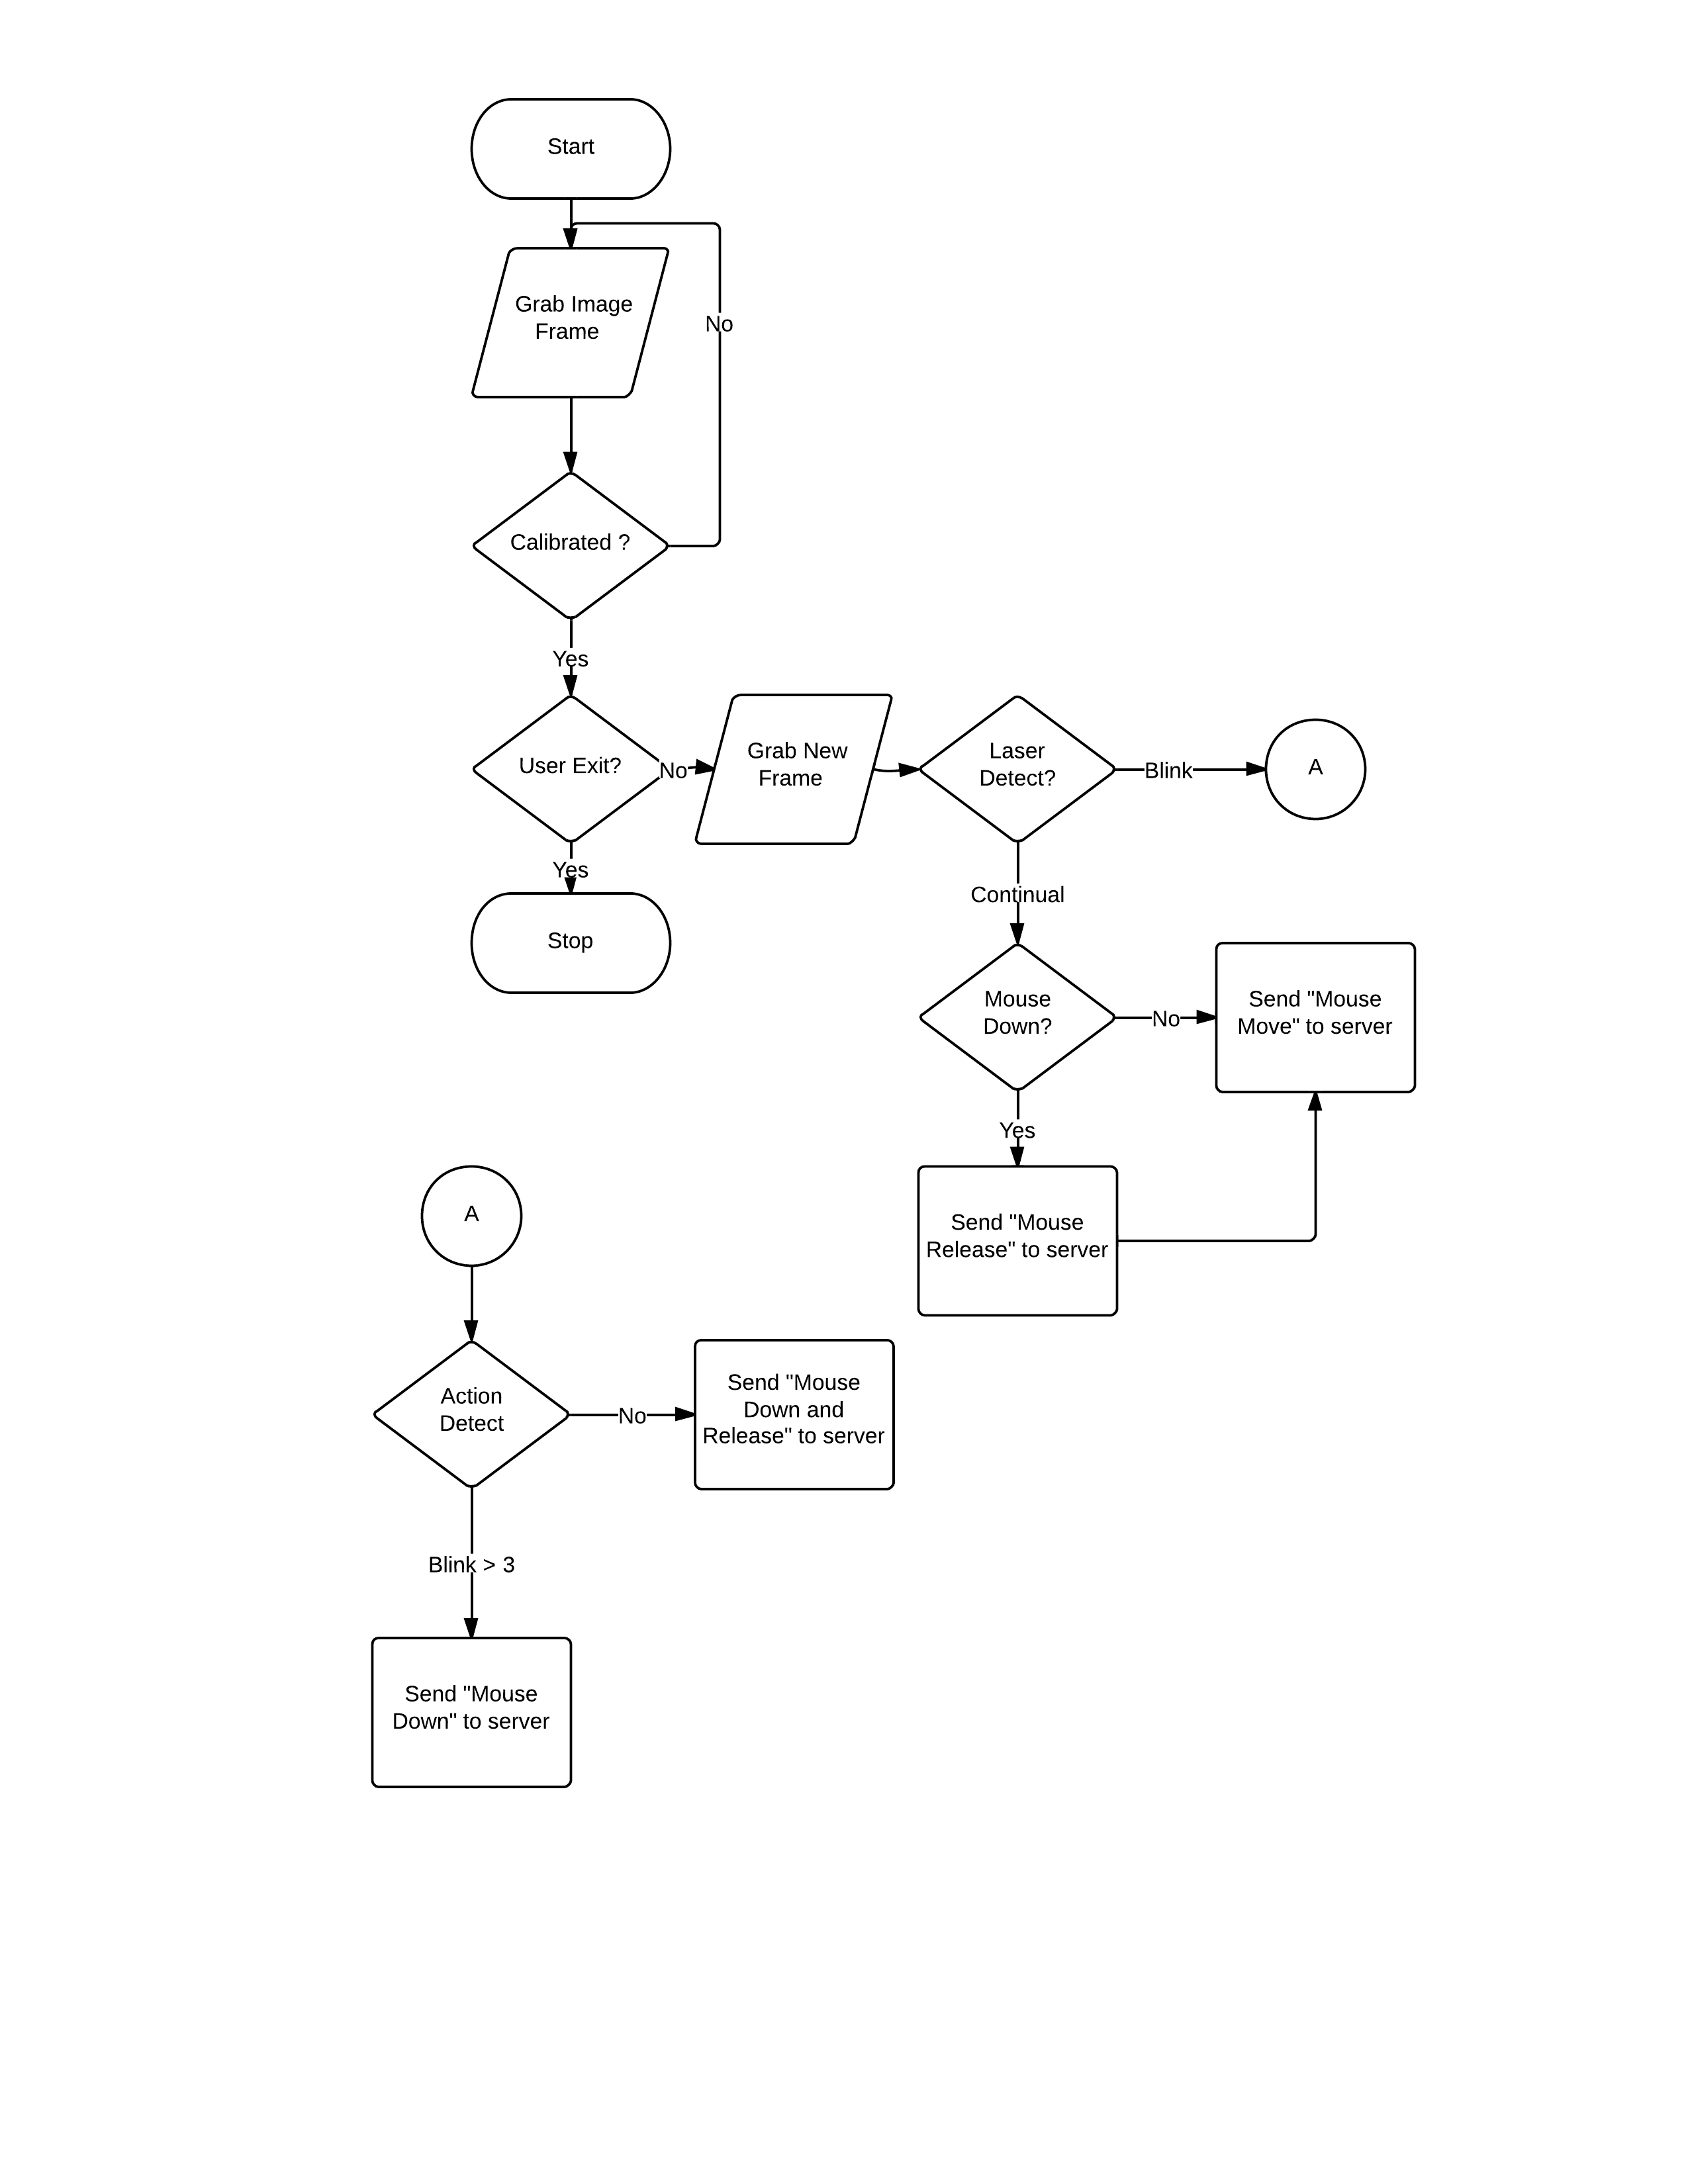
\includegraphics[scale=0.62]{flow.png}
%\\caption{Flow Diagram of System}
%\\label{}
%\\end{figure}
\section{Flowchart of the algorithm}
\begin{appendixfig}
\centering
\tikzstyle{decision} = [diamond, draw, text width=4.5em, text badly centered, node distance=3cm, inner sep=0pt]
\tikzstyle{block} = [rectangle, draw, text width=5em, text centered, rounded corners, minimum height=4em]
\tikzstyle{line} = [draw, -latex']
\tikzstyle{cloud} = [draw, ellipse, node distance=3cm,
    minimum height=2em]
\tikzstyle{circle} = [draw, ellipse, node distance=3cm,
    minimum height=2em]
    
\begin{tikzpicture}[node distance = 2cm, auto]
    % Place nodes
    \node [cloud] (A) {Start};
    
    \node [block, below of=A] (B) {Grab Image Frame};

    \node [decision, below of=B] (C) {Calibrated?};
    
    \node [decision, below of=C, node distance=4cm] (D) {While User Not Exit?};
    
    \node [block, right of=D, node distance=4cm] (E) {Grab New Frame};
    
    \node [decision, right of=E, node distance=4cm] (F) {Laser Detect?};
    
    \node [circle, right of=F, node distance=3cm] (J) {A};
    
    \node [decision, below of=F, node distance=4cm] (G) {Mouse Down?};
    
     \node [block, right of=G, node distance=4cm] (I) {Send "Mouse Move" to Server};
    
     \node [block, below of=G, node distance=4cm] (H) {Send "Mouse Release" to Server};
    
    \node [cloud, below of=D, node distance=4cm] (Z) {Stop};

%\node [circle, below of=Z, node distance=4cm] (K) {A};

%\node [decision, below of=K, node distance=3cm] (L) {Action Detect?};

%\node [block, below of=L, node distance=4cm] (N) {Send "Mouse Down"  to Server};

%\node [block, right of=L, node distance=4cm] (M) {Send "Mouse Down and Release" to Server};


    % Draw edge
%   \path [line] (K) -- (L);            
%    \path [line] (L) -- node {No}(M);
%    \path [line] (L) -- node {Blinks $<3$}(N);
    \path [line] (A) -- (B);
    \path [line] (E) -- (F);
    \path [line] (F) -- node {Blink}(J);
    \path [line] (H) -| (I);
     \path [line] (F) -- node {Continual}(G);
      \path [line] (G) -- node {Yes}(H);
    \path [line] (C) -- node {Yes}(D);
    \path [line] (B) -- (C);
    \path [line] (D) -- node {Yes}(E);
    \path [line] (G) -- node {No}(I);
    \path [line] (D) -- node {No}(Z);
\end{tikzpicture}
\caption{Flowchart of the algorithm}
\end{appendixfig}

\begin{appendixfig}
\centering
\tikzstyle{decision} = [diamond, draw, text width=4.5em, text badly centered, node distance=3cm, inner sep=0pt]
\tikzstyle{block} = [rectangle, draw, text width=7em, text centered, rounded corners, minimum height=2em]
\tikzstyle{line} = [draw, -latex']
\tikzstyle{cloud} = [draw, ellipse, node distance=3cm,
    minimum height=2em]
\tikzstyle{circle} = [draw, ellipse, node distance=3cm,
    minimum height=2em]    
\begin{tikzpicture}[node distance = 2cm, auto]

\node [circle, below of=Z, node distance=4cm] (K) {A};

\node [decision, below of=K, node distance=3cm] (L) {Action Detect?};

\node [block, below of=L, node distance=4cm] (N) {Send "Mouse Down"  to Server};

\node [block, right of=L, node distance=4.5cm] (M) {Send "Mouse Down and Release" to Server};

    \path [line] (L) -- node {Blinks $<3$}(N);
    \path [line] (L) -- node {No}(M);
    \path [line] (K) -- (L);
\end{tikzpicture}
\caption{Flowchart of the algorithm}
\end{appendixfig}
\end{appendices}

\end{document}\documentclass[12pt, a4paper]{article}
